%-----------------------------------------------------
% IBP - Systém pro import/správu fotografií
% Sára Škutová
% xskuto00@stud.fit.vutbr.cz
% 3.1.2017
%-----------------------------------------------------

\chapter{Úvod}
Fotografování nabralo v~posledních letech na nebývalé slávě. Už dávno pominula doba, kdy se pro tvorbu fotografií musel vlastnit drahý fotoaparát. Dnešní, dokonce i~ty levnější modely digitálních fotoaparátu jsou tak schopné, že se o~veškerou těžkou práci dokáží postarat samy, takže stačí jedině zaměřit objektiv a~stisknout tlačítko. Mnoho uživatelů si dnes také vystačí s~mobilním telefonem a~za velmi krátkou dobu mohou vytvořit rozsáhle sbírky fotografií. Se vzrůstajícím počtem fotografií také vzrostl požadavek na jejich správnou archivaci, jenom málokomu se ale chce ručně rozdělovat své výtvory do skupin.

Dalším problémem jsou duplikáty. Velmi často máme na svém mobilním telefonu a~počítači nastavené zálohování, takže se nemusíme obávat o~ztrátu našich velmi cenných dat zaznamenávajících naše zážitky. Díky uložení fotografií na server, lze velmi rychle a pohodlně stáhnout data do počítače. Člověk je ovšem tvor velice zapomnětlivý, a~tak se může stát, že zapomene, zda již dané fotografie stáhl a~zpracoval. Často se pak v~počítači nacházejí duplicitní skupiny fotografií.

Cílem této bakalářské práce je vytvořit aplikaci, která bude automaticky rozdělovat fotografie do skupin a~následně bude vyhledávat jejích duplikáty, které potom umožní uživateli smazat. Toto téma jsem si vybrala, protože mě zajímá tvorba uživatelského rozhrání a~taktéž jsem se chtěla dozvědět něco nového o~fotografiích.

Tento dokument je rozdělen do šesti kapitol. Ve \ref{Digi_foto}.~kapitole bude krátce představen vývoj fotoaparátu a~samotné fotografie. Dále se zde nacházejí základní informace o~tvorbě digitální fotografie a~jaký má na ni informatika pohled. Bude zde vysvětlen termín Exif a~zahrnou se také informace o~nejoblíbenějších a nejpouživatelnějších formátech. \ref{Ex_prg}.~kapitola nabídne výpis a~představení programů, které umožňují rozdělovat fotografie do skupin a/nebo nalézat duplicitní fotografie. Ve \ref{Nvr}.~kapitole lze nalézt návrh funkcí aplikace a~v~\ref{Real}.~se nachází návrh uživatelského rozhraní, návrh testování, implementační popis, představení aplikace, průběh a~výsledky testování. 


\chapter{Digitální fotografie}
\label{Digi_foto}
V~této kapitole lze nalézt krátký souhrn historie vývoje fotografie, dále jak se digitální fotografie tvoří a~co je to datový obraz. V~další části jsou představeny oblíbené typy formátů, do jakých se fotografie ukládají a~v~závěru jsou vysvětleny Exif metadata. Informace uvedené v~této kapitole poskytují pouze základní informace, které mi připadaly zajímavé a~které jsou potřeba k~pochopení probíraného problému, nelze je proto považovat za plný výklad k~problematice. Pokud by se měly sepsat všechny dostupné informace s~jistotou by tento dokument překročil rámec bakalářské práce.

\section{Historie fotografie}
Fotografování se stalo hitem posledních let a~také součástí každodenního života mnoha lidí. Díky rostoucím schopnostem digitálních fotoaparátu a~jejich snižujícím se cenám, se v~dnešní době tvoří více fotografií než kdy jindy. Ke zvyšujícím se počtům také napomáhají oblíbené chytré telefony se zabudovaným fotoaparátem. Ne vždy ovšem existovala tato záplava fotografií.

První \uv{fotoaparáty} byly velice vzdálené dnešním přístrojům. Tyto \textit{camery obscury\footnote{V překladu temná místnost, malý otvor umožňoval v~temné místnosti promítat to co se nacházelo venku, grafické znázornění funkčnosti lze vidět na obrázku \ref{camera_obs_obraz}}} umožňovaly obraz pouze promítat, a~ještě dlouho trvalo, než se vynalezla technologie, která by umožňovala obraz i~zaznamenat \cite{camera_obscura}.

\begin{figure}[h]
\begin{center}
\scalebox{0.5}{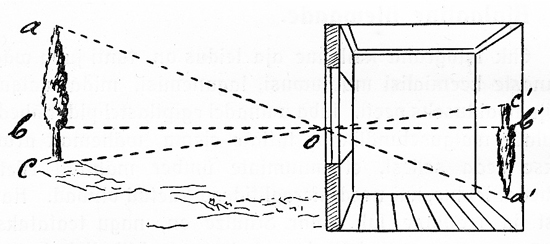
\includegraphics{obrazky-figures/camera_ob.jpg}}
\caption{Funkčnost camery obscury \cite{obrazky_historie}}
\label{camera_obs_obraz}
\end{center}
\end{figure}

První pokusy o~záznam obrazu probíhaly až na přelomu 17. a 18. století, kdy se pomocí chemických látek a~dopadajícího světla na desku podařilo vytvořit první záznam\,--\,fotografii \cite{obrazky_historie}. Tu si lze prohlédnout na obrázku \ref{prvni_foto}.

\begin{figure}[h]
\begin{center}
\scalebox{0.45}{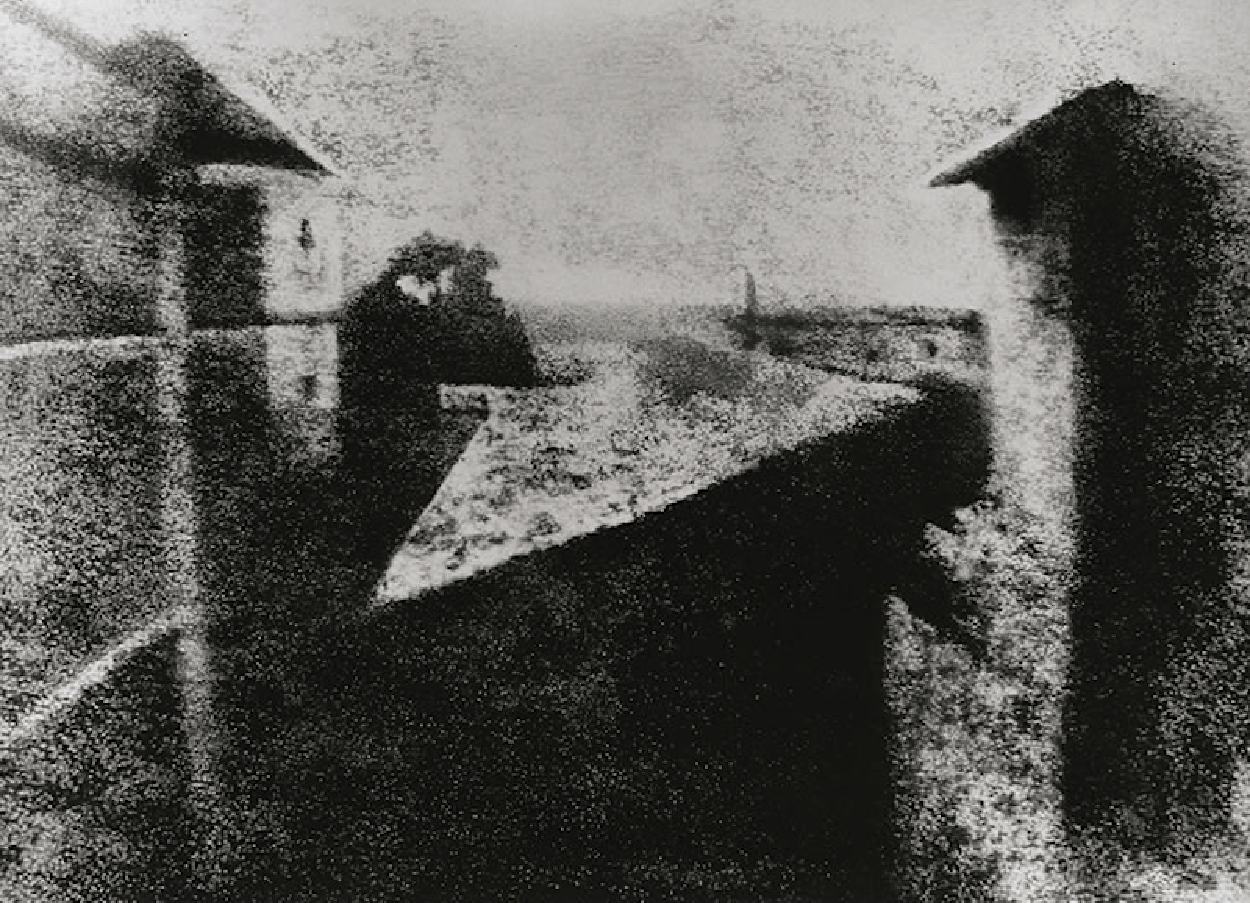
\includegraphics{obrazky-figures/first_photo.pdf}}
\caption{Nejstarší dochovaná fotografie \cite{obrazek_prvni}}
\label{prvni_foto}
\end{center}
\end{figure}

Od té doby se vývoj fotoaparátu a~fotografie významně urychlil. Krátce po prvním záznamu byla vynalezena technika jménem \textit{Daguerrotypie}, která při vyvolávaní používala výpary rtuti. Tato technika umožňovala velice rychle získat požadovaný obraz, když stačila pouze velice krátká doba osvětlení. Jak se ovšem zmiňuje v~druhé kapitole zde \cite{obrazky_historie}, nevýhodou této techniky bylo, že daný obraz byl velice citlivý na dotek, nešel kopírovat a~použité látky byly vysoce toxické.

Dalším důležitým vynálezem byly kolodiové negativy, také známe jako \uv{mokrý proces}. Tato technika umožňovala kvalitní mnohočetné kopírování a~obrazy byly ostré s~množstvím detailů, ale musely se zhotovit hned a~ve tmavé místnosti. I~přes tyto nedostatky začala vrůstat oblíbenost fotografování a~s~tím i~počet fotografií.

Dalším objevem, který negoval mokrý proces, byl \uv{suchý proces}, který používal bromostříbrné negativy. Ačkoliv se tato technika ve svých počátcích potýkala s~problémy\,–-\,malou citlivostí a~většího zrna, po nějaké době se kvalita zlepšila a~suchý proces se začal upřednostňovat. Co je důležité, tak dle \cite{obrazky_historie} se díky této technice mohly fotografie začít průmyslové vyrábět což opět zvýšilo oblíbenost fotografování.

Černobíle fotografie, ale nestačily na zachycení barevného světa, a~tak aby se uchoval zájem lidí, začal vývoj barevných snímků. První technika se dle třetí kapitoly v~\cite{obrazky_historie} objevila již na začátku 20.~století\footnote{První barevná fotografie vznikla dříve (v~roce 1861) vyfotografováním objektu s~různými barevnými filtry a~následným naložením vrstev na sebe, k~vidění na obrázku \ref{prvni_barev_foto}} a~nazývala se \textit{Autochrom}.
Výroba těch fotografií byla ovšem náročná, a~navíc se z~nich nedalo dělat kopie.

\begin{figure}[ht]
\begin{center}
\scalebox{0.6}{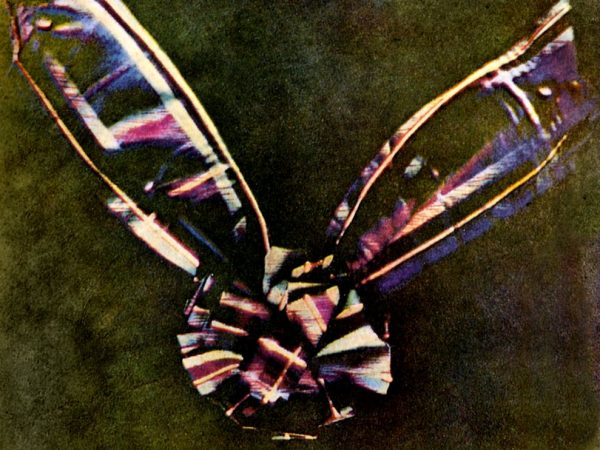
\includegraphics{obrazky-figures/first_color_photo.jpg}}
\caption{První barevná fotografie \cite{obrazek_barev_prvni}}
\label{prvni_barev_foto}
\end{center}
\end{figure}

V~té tobě se také začaly vyrábět fotoaparáty se svitkovým filmem, který rozšířil fotografování i~k~méně zdatným lidem, protože po zaplnění všech svitků je stačilo pouze odeslat k~výrobci fotoaparátu a~ten vyvolané fotografie poslal zpět k~uživateli.

V~roce 1908 byl přihlášen patent s~prvním barevným filmem, který se skládá z~tří světlocitlivých vrstev (modrá, zelená a~červená) a~barvotvorných chemikálií, které v~průběhu vyvolávaní měnily barvu.

Dalším důležitějším objevem byla v~roce 1963 firmou Polaris vyvinuta emulze, která umožňovala tvořit okamžité fotografie \footnote{Fotografie, které se na snímku objevili několik minut po expozici a~nepotřebovaly žádné další zpracování}.

Díky všem těmto vynálezům se počet fotografií pomalu zvyšoval, a~když pak v~roce 1975 \cite{prvni_digi} byl vytvořen první digitální fotoaparát, tak se odstartovala doba, která pokračuje až do dnešních dnů, kdy se fotografování stalo součástí života mnoha lidí.

\section{Tvorba digitální fotografie}
Fotografie lze překládat jako kresba světlem a~jak u~klasické fotografie, tak i~u~digitální platí, že obraz se nejprve zachytí objektivem a~následně dopade na záznamové médium. V~klasických fotoaparátech bylo tímto médiem světlocitlivý film, kdežto v~digitálních tuto úlohu plní elektronický světlocitlivý snímač/čip. Tady ovšem práce digitálního fotoaparátu nekončí, intenzita signálů z~jednotlivých buněk snímače jsou dále zpracovávána A/D (analogově/digitálním) převodníkem, výchozí data procházejí firmwarem daného výrobce fotoaparátu a~až potom je fotografie uložena na paměťové médium. Oproti tomu u~klasického fotoaparátu plní záznamové médium (film) i~úlohu archivačního média \cite{digi_foto_book}. 

\subsection*{Snímač digitálního fotoaparátu}
Snímač je tvořen maticí světlocitlivých buněk. Počtem buněk lze určit kolik bude mít výsledná fotografie pixelů, jak bude kvalitní a~kolik bude obsahovat detailů. Ne vždy ovšem vysoký počet pixelů (lépe spíš Megapixelů) znamená kvalitnější fotografii. Dalším důležitým parametrem je to, jak velkou snímací plochu čip má, v~případě, že je na malé ploše nahuštěno až příliš mnoho pixelů, tak je jejich plocha mnohem menší, a~proto zaznamenávají méně kvalitně. Ve výsledku je pak nekvalitní fotografie s~vysokým stupněm šumu \cite{pixely}.

Ačkoliv by se mohlo zdát, že snímač zachycuje celý obraz, tak to není pravda. Samotný čip zachycuje pouze intenzitu světla. Podle množství světla se následně vybudí odpovídající signál a~následné zpracování se přenechá další elektronice fotoaparátu. Barevnosti se docílí pomocí barevných filtrů, které jsou umístěny před buňkami snímače\,--\,tzv. \textit{Bayerova maska} (k~vidění na obrázku \ref{filtry}). Většinou se používají filtry z~RGB modelu (o~něm v~další kapitole), při čemž zelené barvy je více kvůli tomu, že lidské oko je nejvíce citlivé právě na tuto barvu \cite{maska_barva}. Pixel tak nese informaci o~jedné barvě z~RGB modelu. V~dalším kroku pak interpolační algoritmus přečte data ze sousedních buněk a vypočítá finální barvu.

\begin{figure}[ht]
\begin{center}
\scalebox{0.45}{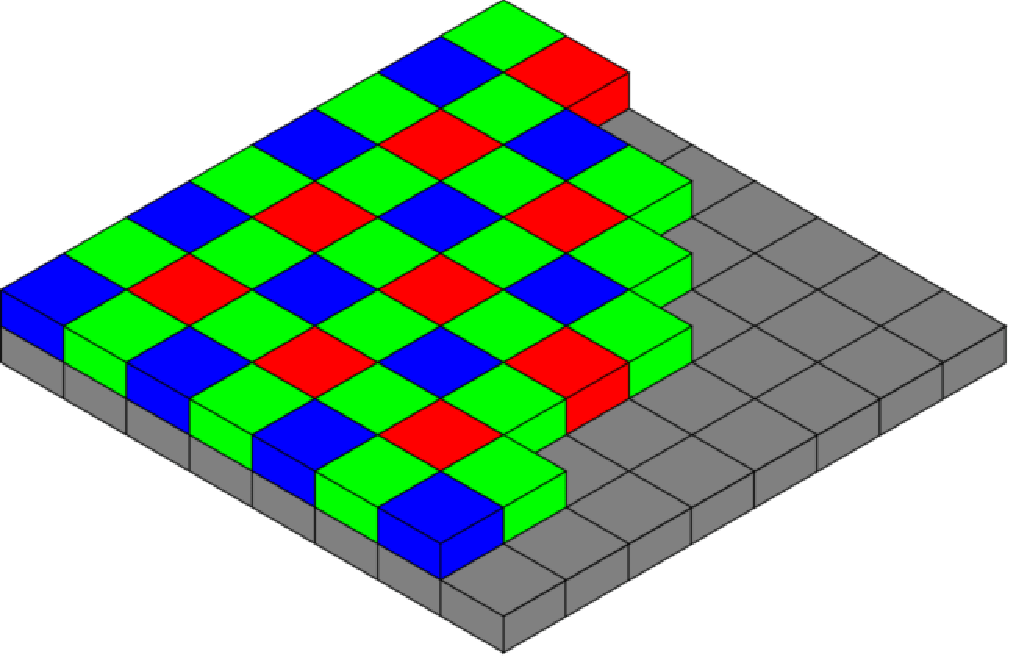
\includegraphics{obrazky-figures/maska_snimac.pdf}}
\caption{Bayerova maska na snímači (šedá barva) \cite{maska_barva}}
\label{filtry}
\end{center}
\end{figure}

Za snímačem data zpracovává AD převodník, který převede napěťový signál (který, jak bylo zmíněno dříve, se generuje po dopadu světla na snímač) do binární podoby. Následně jsou digitální data zpracovává procesorem a~firmwarem daného výrobce dle nastavení fotoaparátu a~poté uložena na paměťové médium ve zvoleném formátu \cite{digi_foto_book}.

\section{Digitální obraz a barevné modely}
Z pohledu matematicky lze na digitální obraz pohlížet jako na spojitou funkci \ref{spoj_funk}, které se také říká obrazová funkce. Z pravidla pak lze říci, že výsledky obraz je maticí bodů z dané funkce. Hodnoty těchto bodů pak odpovídají nějaké fizikální veličině \cite{obraz_mat}.

\begin{equation}
\label{spoj_funk}
f(x,y)
\end{equation} 

Co se týče reprezentace zpracovávaného obrazu tak na něho lze v~počítačové grafice nahlížet dvojím způsobem\,--\,\textbf{rastrově} a \textbf{vektorově} \cite{IZG_opora}.

\subsection*{Rastrová grafika}
Obraz je popsán pomocí mřížky (matice) jednotlivě barevných bodů (pixelů). Každý pixel je popsán svou polohou a~barevnou informací, kterou v~sobě uchovává. Platí, že čím více pixelů, tím detailnější obrázek, ovšem s~jejích vzrůstajícím počtem se také zvětšují paměťové nároky na uložení výsledného obrazu. Na kvalitu má vliv také barevná hloubka \footnote{Označuje kolik bitů se použije k~uložení barvy v~každém kanálu používaného barevného modelu}. Při nesprávném zobrazení (přílišné přiblížení) se mohou zobrazit jednotlivé pixely \cite{rastr_vektr}.

\subsection*{Vektorová grafika}
Obraz je popsán pomocí jednotlivých objektů (bodů, přímek, křivek), samotné objekty jsou pak popsány souborem instrukcí. Vektorový obrázek lze jakkoliv přibližovat bez ztráty kvality \cite{rastr_vektr}.

\begin{figure}[h]
\begin{center}
\scalebox{1.5}{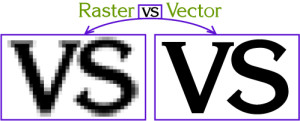
\includegraphics{obrazky-figures/raster_vektor.jpg}}
\caption{Rozdíl mezi rastrovou a~vektorovou grafikou \cite{rastr_vektr_obr}}
\label{rastr_vektor_label}
\end{center}
\end{figure}

Rastrová grafika se ve většině případů používá jako reprezentace digitální fotografie a~v~televizi. S~vektorovou grafikou se lze setkat při tvorbě ilustrací, diagramů a počítačových animací. Grafický rozdíl mezi rastrem a~vektorem si můžete pohlédnout na obrázku \ref{rastr_vektor_label}.

K~popisu barev se v~počítačové grafice používají barevné modely. Díky nim lze pomocí několika základních barev namíchat požadovanou barvu. Na následujících řádcích jsou popsány nejpoužívanější barevné modely.

\subsection*{RGB model}
Nejznámější a~nejvíce používaný model. Právě s~ním pracují digitální fotografie. Jedná se o~aditivní model, což znamená, že se jednotlivé barevné složky sčítají ve výslednou barvu. Toho například využívají monitory a~displeje kde se barvy tvoří pomocí přičítání tří světelných kuželů s~odpovídajícími barevnými filtry k~černé barvě monitoru \cite{barvy}.

\begin{figure}[h]
\begin{center}
\scalebox{0.6}{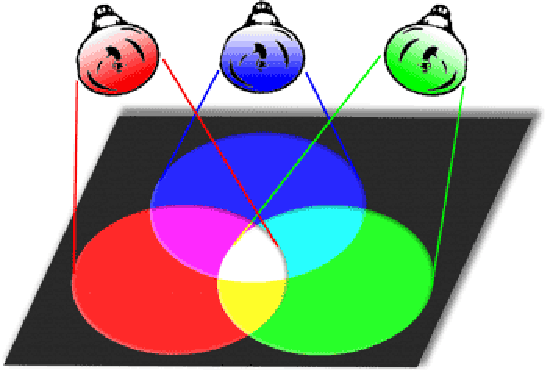
\includegraphics{obrazky-figures/rgb_monitor.pdf}}
\caption{ Aditivní model\,--\,sčítání barev na tmavé ploše \cite{rgb_monitor}}
\label{rgb_monitor_obraz}
\end{center}
\end{figure}

V~tomto modelu jsou tří základní barvy\,--\,červená, zelená a~modrá. Právě na tyto barvy je lidské oko nejvíce citlivé. Další barvy se pak získávají jejích kombinací a~intenzitou světla. U~digitální fotografii (a~v~počítačové grafice taktéž) se nejmenší intenzita světla reprezentuje hodnotou 0 a~maximální hodnotou 255 (to platí pouze v~případě, že je použita 8-bitová barevná hloubka) \cite{rgb_monitor}.
Model RGB lze graficky vyjádřit taktéž jako krychli, jak jde vidět na obrázku \ref{rgb_krychle_obraz}.

\begin{figure}[h]
\begin{center}
\scalebox{0.7}{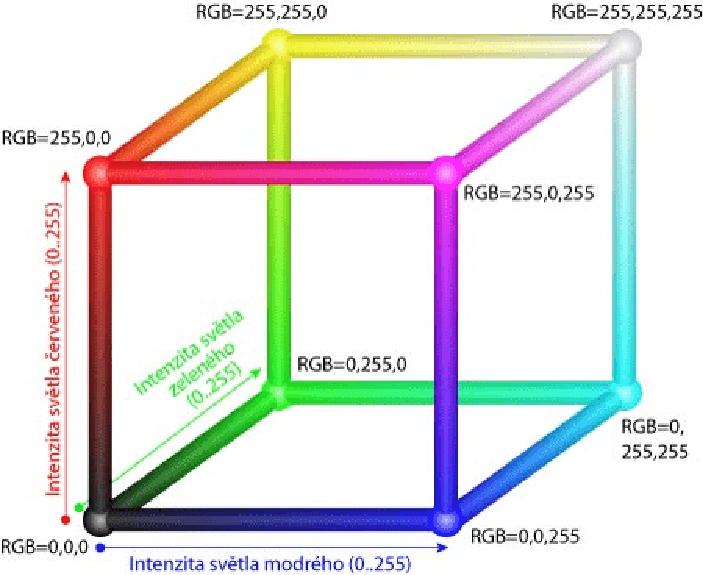
\includegraphics{obrazky-figures/rgb_krychle.pdf}}
\caption{Grafické znázornění RGB modelu\cite{rgb_monitor}}
\label{rgb_krychle_obraz}
\end{center}
\end{figure}

\subsection*{CMYK model}
Tento model je subtraktivní model, což znamená, že se jednotlivé barvy odečítají. Lze také říct, že se s~každou barvou ubírá část světla\,--\,jak světlo prochází barevnými složkami, tak je stále více pohlcováno. Používá se hlavně v~tiskárnách při míchání pigmentů. Problémem je, že ne všechny barvy z~RGB modelu, lze převést do CMYK a naopak, a~z~toho důvodu se pak stává, že vytisknutá fotografie má na papíře menší barevnou kvalitu než na monitoru \cite{barvy}.

\begin{figure}[hb]
\begin{center}
\scalebox{0.6}{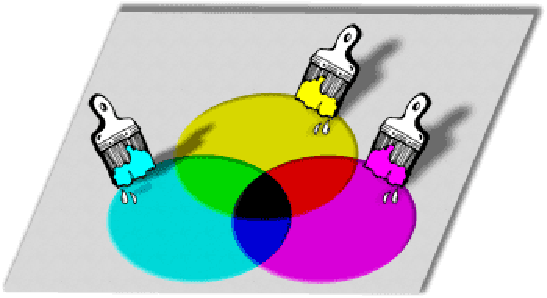
\includegraphics{obrazky-figures/cmyk.pdf}}
\caption{CMYK model\cite{rgb_monitor}}
\label{cmyk_obraz}
\end{center}
\end{figure}

Základními barvami v~tomto modelu jsou: azurová (C\,--\,Cyan), purpurová (M\,--\,Magenta) a~žlutá (Y\,--\,Yellow). Ovšem velmi často se k~těmto barvám přidává čtvrtá a~to černá (K\,--\,blacK), a to z~důvodu, že při běžném použití v~tiskárnách kombinace CMY nestačí na vytvoření kvalitní černé barvy. Černá funguje také jako podpora k~vytvoření tmavých barev a~k~ušetření ekonomických nákladů \cite{rgb_monitor}.

\section{Datové formáty}
Po zpracování fotografie softwarem fotoaparátu, musí být fotografie uložena do nějakého datového formátu. Pro připomenutí, jak už bylo psáno dříve, fotografie se skládá z~pixelů a~každý pixel si pamatuje jakou barvu obsahuje. Pro reprezentaci barev ve fotografiích se používá RGB model, což znamená, že jeden pixel obsahuje 3~barevné složky pro zakódování své barvy. Barevná hloubka určuje, kolik bitů se použije pro zakódování barvy v~každé složce. Čím více bitů tím více barev je možné vytvořit. Datové formáty pak určují, jak se fotografie uloží a~kolik zabere paměťového místa.

\subsection*{JPEG}
JPEG je nejrozšířenějším datovým formátem. Používá se nejen k~uložení digitálních fotografií, ale také i~obrázků. Jeho název je ve skutečnosti zkratka od \textit{Joint Photographic Experts Group}, což je název komise, která v~roce 1992 tento standart vytvořila. Svou oblíbenost si získal díky tomu, že umožňuje uložit obrázky, tak aby výsledná velikost souboru byla co nejmenší, bez změny velikosti (šířky a výšky) původního obrazu. Menší velikost také umožňuje rychlejší zpracování fotografie softwarem aparátu a~rychlejší uložení, díky čemuž lze rychleji tvořit další fotografie (druhý díl v \cite{datove_formaty_web}). JPEG také podporuje ukládání Exif metadat (tyto metadata se popisují v~sekci \ref{Exif_metadata}).

Používá ztrátovou kompresi\,–-\,odstraňuje jemnější detaily fotografie (slučuje podobně barevné pixely), cílem je ovšem získat obraz, který by lidské oko nebylo schopné odlišit od originálu. Každopádně při kompresi dochází k~degradaci kvality fotografie a~v~případě příliš velké komprese se začnou objevovat defekty\,–-\,vzniknou plochy a~pruhy bez hladkých přechodů \cite{digi_foto_book2}.

Ve většině editorů, které se JPEG pracují, je možné nastavit přesnou míru komprese (v~procentech). U~digitálních fotoaparátu lze většinou pouze nastavit jistý stupeň, při čemž každý výrobce může mít odlišné nastavení.

JPEG má ovšem i~své nedostatky (viz. třetí díl z~\cite{datove_formaty_web}). Pracuje vždy pouze v~8-bitové barevné hloubce, nepodporuje průhlednost a~animaci, nelze ukládat obrázek s~více vrstvami. Komprese bude vždy ztrátová a~v~případě, že se obrázek opakovaně upravuje a~opětovně ukládá do formátu JPEG, tak postupně dochází k~degradaci jeho kvality.

\subsection*{JPEG 2000}
Tento formát lze nazývat pokračovatelem klasického JPEGu. Značně vylepšuje kompresní algoritmus, který již nepracuje s~částí obrazu, ale s~celým obrazem najednou. Díky tomu umožňuje o~20-30\,\% lepší kompresní poměr.

Oproti svému předchůdci, JPEG 2000 nepodporuje ukládání Exif metadat, na druhou stranu ale umožňuje ukládat průhlednost i~práci s~větší barevnou hloubkou. Podporuje také bezztrátovou kompresi.

Ačkoliv byl JPEG 2000 vytvořen na začátku tohoto milénia a~zdá se být lepší alternativou k~JPEG, tak do dnes se nepodařilo rozšířit jeho používání \cite{JPEG2000}.

\subsection*{TIFF}
Tento formát býval v~minulostí velmi používanou alternativou k~JPEG. Název je zkratkou od \textit{Tagged Image File Format} a~původně sloužil k~ukládání obrázků ze skenování.

Je to velmi flexibilní formát, který také slouží jako kontejner (umožňuje přenášet různá obrazová data). To, co je uloženo v~kontejneru, je popsáno v~hlavičce TIFFu v~podobě tagů. Díky tomu lze například rozpoznat s~jakou barevnou hloubkou se pracuje, jaký je použit způsob komprese, jak velký je soubor. Umožňuje také kombinovat různé obrázky v~jednom souboru. Ovšem neexistuje standart, který by vynucoval, jaké tagy se mohou použít a~v~jakém pořadí. Tato svoboda umožňuje, že některé programy nebudou schopny daný soubor přečíst a porozumět (viz. sedmý díl ze série \cite{datove_formaty_web}).

Dále se také v se v sedmém díle z \cite{datove_formaty_web} píše, že TIFF může pracovat i~bez komprese, v~tom případě, ale výsledný soubor bude velmi veliký a~jeho ukládání pomalé, i~přesto však digitální fotoaparáty umožňuji ukládat fotografie do tohoto formátu.  Lze také použít bezztrátovou i~ztrátovou kompresi a~oproti JPEG je také schopen pracovat s~různými barevnými hloubkami či s~odlišnými barevnými modely. Mezi další výhody patří, že umožňuje ukládat obrázky s~vrstvami, podporuje ukládání Exif metadat a~dokáže uchovávat průhlednost.

Tento datový formát se doporučuje, pokud se požaduje fotografie v~stoprocentní kvalitě. V~praxi ale není příliš velký rozdíl mezi obrázkem ve formátu TIFF a~JPEG v~nejvyšší kvalitě, a~navíc se více doporučuje formát RAW, který TIFF defacto nahradil (viz. osmý díl ze série \cite{datove_formaty_web}) .

\subsection*{RAW}
Obrazový formát RAW lze prakticky využít jako velmi dobrou alternativu k~formátu TIFF. Název pochází od anglického slova \textit{raw} (surový, hrubý) a~přesně vystihuje celý formát\,–-\,data neprošla jakoukoliv úpravou, žádným upravujícím algoritmem a~jsou uložena v~surovém stavu přímo ze snímače.

Naneštěstí neexistuje standart, který by podobu RAW formátu nějak formalizoval. Z~toho důvodu si každý výrobce digitálních fotoaparátu tvoří svůj vlastní formát. Firma Adobe se pokusila o~standardizaci, ale zatím neúspěšně \cite{RAW1}. 

Díky tomu, že data pocházejí přímo ze snímače, tak RAW soubory mají menší velikost než TIFF fotografie. Mezi další výhody patří, že před vyvoláním fotografií, lze doopravit různá technická data, která ovlivňuji výslednou kvalitu fotografie\,–-\, expozici, vyvážení bíle apod.~Společně se surovými daty se ukládají i~Exif metadata \cite{RAW_celkove}.

Nevýhodou RAW je, že fotografie v~tomto formátu nelze okamžitě zobrazit. Pro jejích prohlížení a~vyvolání jsou potřeba specializované programy. A~navíc výsledná velikost soubore je mnohem větší než fotografie v~JPEG formátu, čím se také zvyšuje doba potřebná k~jejích zpracování a~uložení \cite{RAW2}.

Celkově se RAW doporučuje použít pouze v~případě, že chceme mít fotografie v~nejlepší kvalitě, a~nefotíme sekvenční snímky.

\section{Informace o~fotografii\,--\,Exif metadata}
\label{Exif_metadata}
Každý digitální fotoaparát, ale také digitální kamery a~některé skenery, ukládají k~vytvořeným obrázkům dodatečná data\,–-\,metadata. Na následujících řádcích lze najít základní informace o~Exif standartu, který je nejvíce asociován s~digitálními fotografiemi.

Exif je zkratka od \textit{Exchangeable Image File Format} a~tento standart byl v~roce 1995 vytvořen japonskou společností JEIDA (nyní JEITA). Naštěstí se na něm pracuje dodnes, a~nejnovější verze, s~označením 2.31, byla vydána v~roce 2016. Tyto metadata jsou připojována k~výslednému snímku a~obsahují informace o~fotografií a~také o~nastavení fotoaparátu v~době tvoření obrázku. Díky tomu lze z~digitální fotografie zjistit nejenom datum a~čas vytvoření, ale také technické informace jako zda byl použit blesk či jaká je použita komprese. Uložené informace mají podobu tagů \cite{EXIV_standart}.

Tyto metadata lze později na počítači číst, modifikovat i~celkově smazat. Mazání Exif metadat se doporučuje, v~případě, že chceme fotografie publikovat online, z~důvodu bezpečnosti na internetu, když některé z~tagů uchovávají i~GPS polohu místa kde se daná fotografie vytvořila\cite{EXIV_remove}. Některé webové stránky při nahrání fotografie mažou EXIF metadata automaticky, např. Facebook. Další nechtěné smazání se může stát v~případě, že se pracuje s~editorem, který neumí pracovat s~Exif daty. Při editaci tagů lze také přidat jméno autora, komentář nebo i~vodoznak. Tyto dodatečné informace umožňují automaticky uložit i~některé fotoaparáty. Kromě informací o~nastavení přístroje v~době tvorby fotografie se ukládá také malý náhled na výslednou fotografii, díky němuž ji lze mnohem rychleji zobrazit, než kdyby se měly načíst všechny pixely.

Kromě standartních tagů mohou výrobci digitálních fotoaparátu přidávat i~své vlastní tagy, to ovšem může způsobovat, když programy pro čtení metadat nebudou schopny tyto dodatečné informace přečíst.

Ukládaní Exif metadat podporují obrazové formáty JPEG, TIFF, RAW. Oproti tomu ve formátech JPEG 2000, GIF, nebo PNG tyto data nenaleznete \cite{datove_formaty_web}.

\section{Technologie pro tvorbu}

Programy pro správu fotografií se objevují na všech oblíbených platformách (Windows, Linux, Mac) a~můžou naprogramovány pomocí velkého množství prostředků. Při správném výběru technologie je pak možné velmi jednoduše přenést aplikaci z~jedné platformy na druhou.

\subsection*{C++}

C++ je oblíbený programovací jazyk a~v~dnešní době jeden z~nejvíce používaných s~širokou škálou podpory. Používá se nejenom na tvorbu desktopových aplikací, ale také na tvorbu her, mobilních nebo také webových aplikací. Tento jazyk byl pro tuto práci vybrán z~toho důvodu, že je schopen velmi rychle provést určené úkony. Tato vlastnost se velmi hodí do tohoto projektu, protože se zde bude pracovat s~velkým množstvím souborů, které se musí otevřít, přečíst a případně porovnat. C++ má ovšem i~své stinné stránky\,–-\,neobsahuje automatickou správu paměti, takže se programátor sám musí postarat o~to, aby vytvořené objekty správně odstraňoval, také na příklad má delší učící křivku, což některé začínající programátory může odradit.

\subsection*{Knihovna Exiv2}

Tato knihovna byla vytvořena pro práci s~metadaty fotografií. Umožňuje je extrahovat, přidávat, modifikovat nebo i~mazat. Podporuje také širokou škálu datových formátů fotografií. Pro tento projekt byla vybrána z~důvodů toho, že je napsaná v~jazyce C++ a~také proto, že je svými vývojáři stále podporována a~stále ve vývoji. Kromě toho, že lze použít jako knihovna do programu, tak také existuje ve verzi jako utilita do příkazové řádky. Více informací o~této knihovně lze najít zde \cite{EXIV_knihovna}.

\subsection*{Qt framework}

Qt je multiplatformní framework \cite{Qt}, který umožňuje vytvářet rozsáhle aplikace s~moderním grafickým uživatelským rozhraním. Díky tomu může být stejná aplikace bez problému přeložena na různých operačních systémech bez jakéhokoliv upravování. Lze použít se zdarma licenci nebo s~placenou. Pro tento projekt by vybrán, protože umožňuje lehce vytvořit uživatelské rozhraní, které bude mít vždy nativní vzhled k~danému operačnímu systému.



\chapter{Existující programy}
\label{Ex_prg}
Tato kapitola popisuje několik programů, které se zaměřují na správu sbírek fotografií, automatické vytváření skupin a~vyhledávání jejích duplicit. Při vybírání softwaru, byl kladen důraz na to, aby byly zdarma a~umožňovaly používat požadované funkce i~ve svým základních verzích. 

\section{Programy pro rozdělování do skupin}

Následující programy obecně pro rozdělování využívají 2~principy, a~to vytvoření skupin (lze také označovat jako album) podle umístění, kdy všechny fotografie z~dané složky jsou uloženy do jedné skupiny anebo podle informací z~Exif metadat.

\subsection*{Adobe Bridge CC}

Program Adobe Bridge CC od firmy Adobe \cite{AdobeBridge} slouží jako správce souborů mezi jinými i~fotografií. Používá se jako doplňková služba pro ostatní programy ze série Creative Cloud od Adobe, ale lze s~ním pracovat i~odděleně. Hlavní okno aplikace lze vidět na obrázku \ref{adobe_b}.

\begin{figure}[h!]
\begin{center}
\scalebox{0.49}{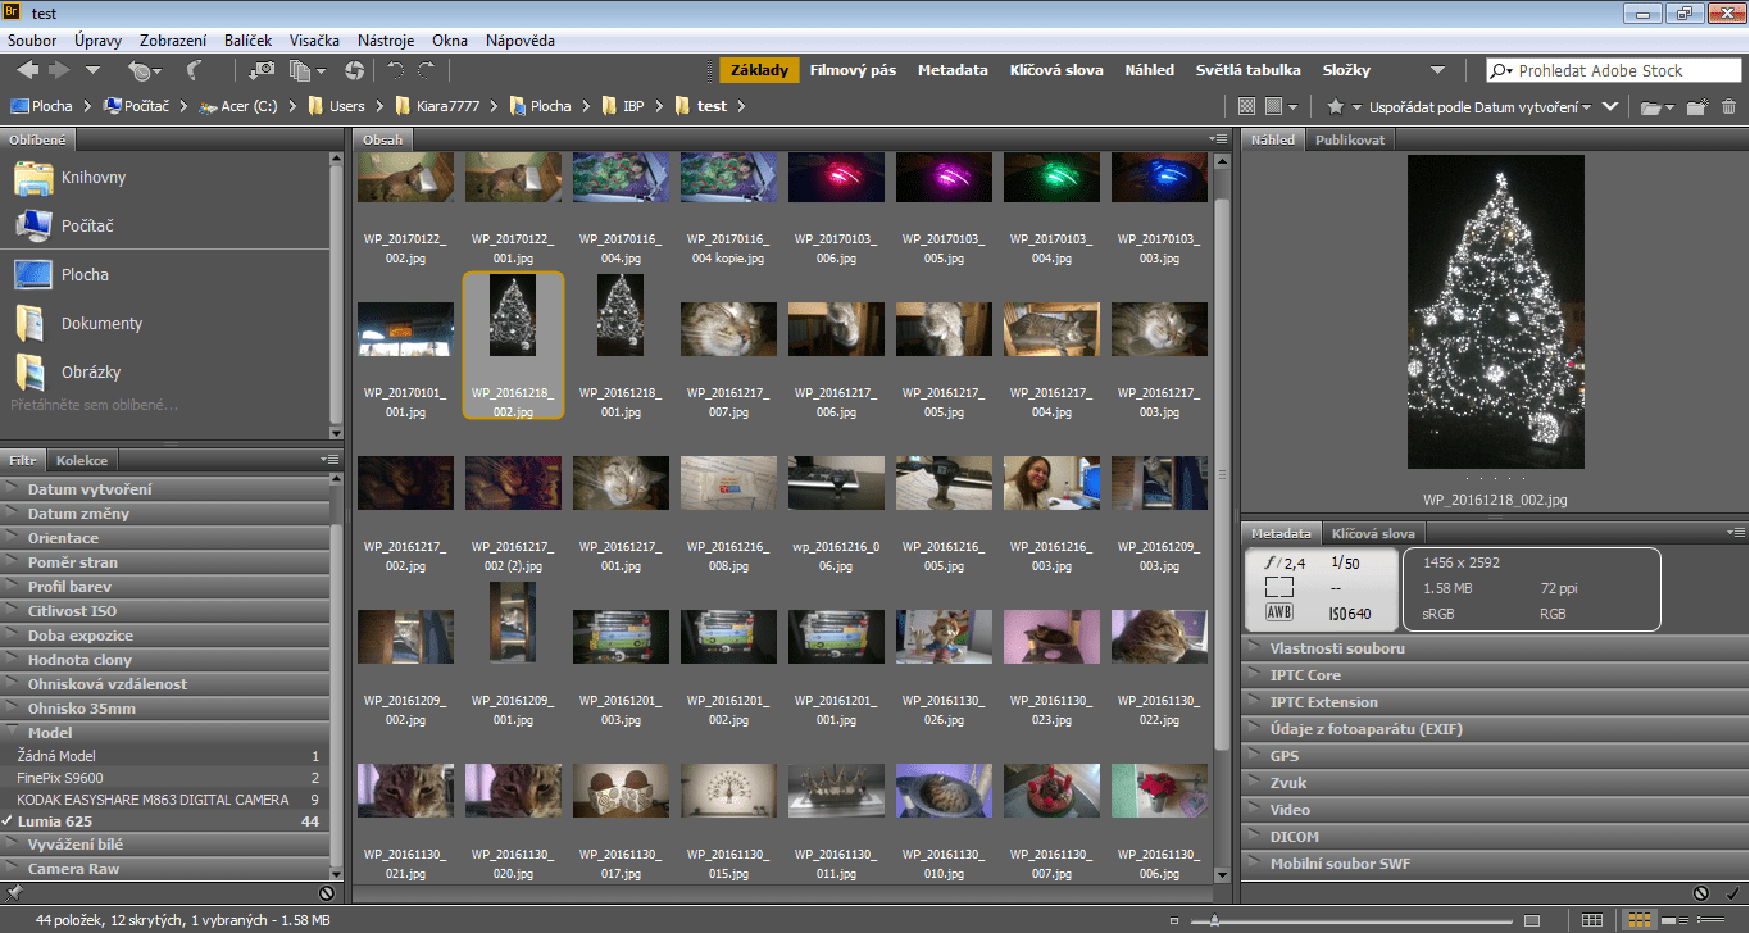
\includegraphics{obrazky-figures/AdobeBridgeCC.pdf}}
\caption{Hlavní okno programu Adobe Bridge CC}
\label{adobe_b}
\end{center}
\end{figure}

Tento program umožňuje zobrazit soubory/fotografie umístěné v~jednotlivých složkách. Dále obsahuje také funkce pro načtení fotografií z~digitálního fotoaparátu. Při importu lze nastavit automatické roztřídění do podsložek podle datumu vytvoření fotografie, automatické přejmenování dle vzoru nebo přidělit základní metadata obsahující informace o~tvůrci fotografie. Dále lze importované fotografie smazat ze zdroje a vytvořit záložní kopie.

Při kliknutí na fotografií na pravé straně zobrazí její náhled a~pod ním lze procházet jednotlivá metadata. Tyto data lze prohlížet, a~některá z~nich lze smazat nebo editovat. Také se zde mohou přiřadit dodatečné informace, které většina fotoaparátů nepřidává\,–-\,informace o~autorovi, popis fotografie, klíčová slova a~mnohem více.

Mezi další schopnosti tohoto programu patří zobrazování skupin fotografií podle zaznačené kategorie.  Toho lze docílit pomocí filtrů. Na obrázku \ref{adobe_b} lze vidět, že byla zaznačena kategorie pro určitý model digitálního fotoaparátu. Jednotlivé kategorie lze kombinovat.
V~této části programu, lze také vytvářet kolekce (vlastní skupiny) nebo lze využít funkce Smart kolekce, která dle rozličných kritérií, které se dají i~kombinovat, vytvoří požadovanou skupinu. Vytvořenou kolekci lze pak dále upravovat.

Adobe Bridge CC je ale pouze správcem souborů, a~proto neobsahuje funkce pro grafické upravování digitálních fotoaparátu.

\subsection*{Phototheca}

Správce fotografií Phototheca od firmy Lunarship Software \cite{Phototheca} je další program, který umožňuje při importu fotografií jejích rozdělení do skupin (zde nazvaných jako Events). Hlavní okno aplikace s~již vytvořenými událostmi si lze prohlédnou na obrázku \ref{phototh_ob}.

\begin{figure}[h!]
\begin{center}
\scalebox{0.49}{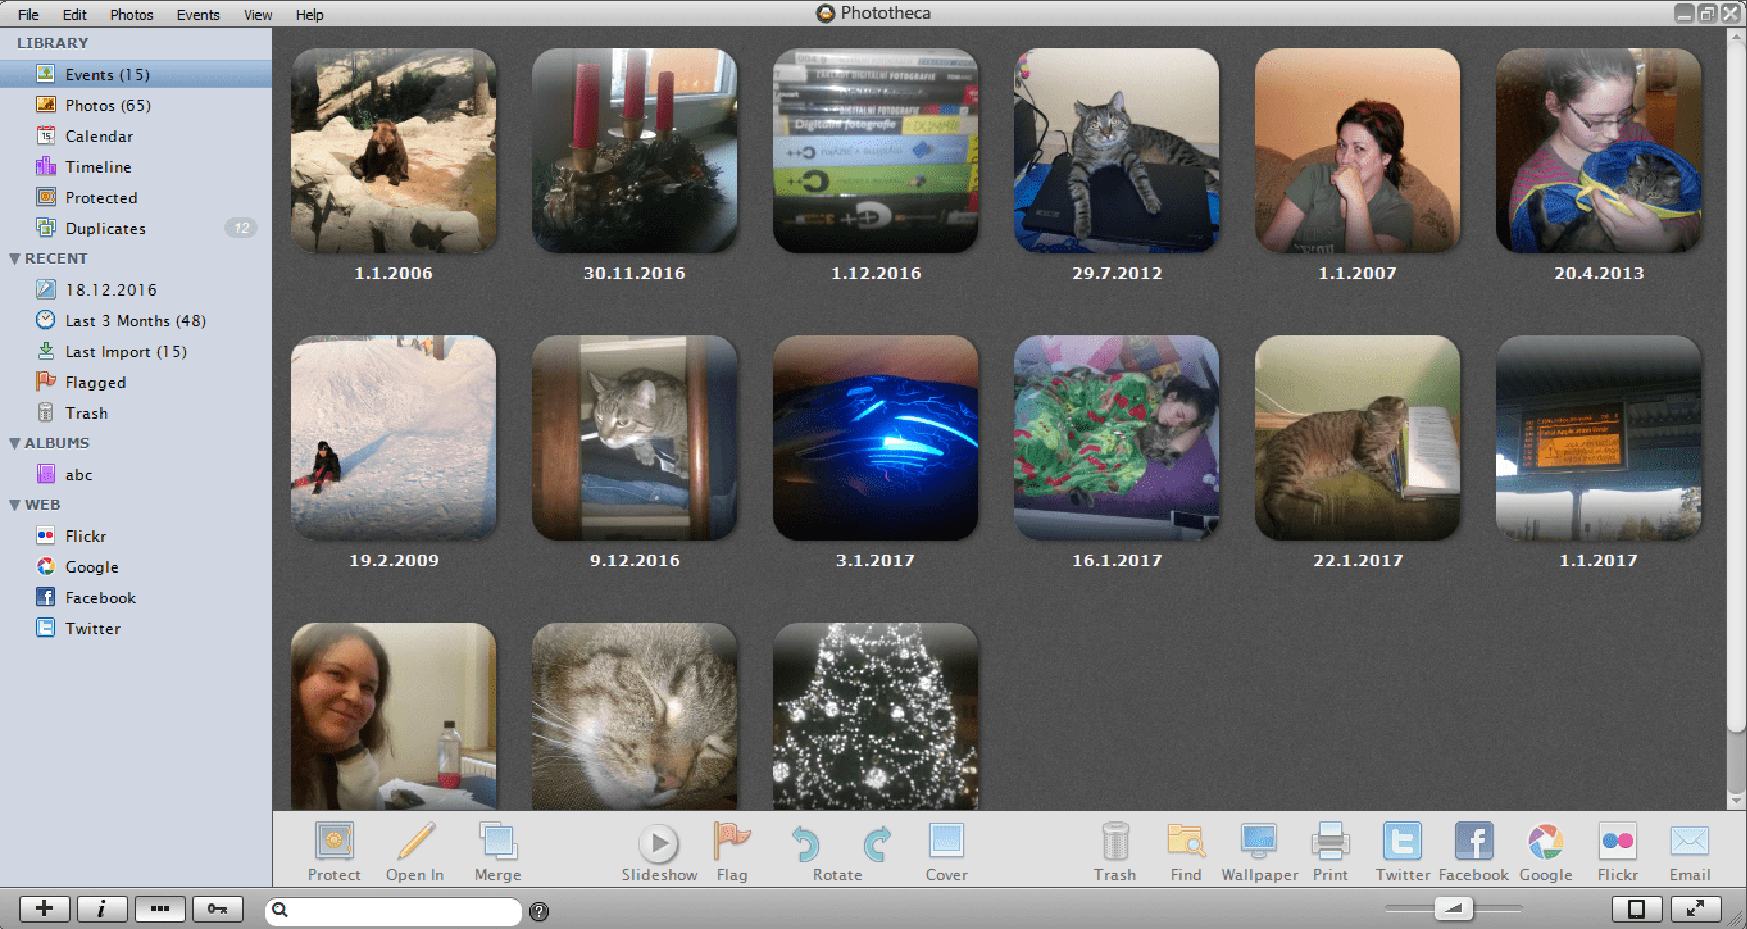
\includegraphics{obrazky-figures/Phototheca.pdf}}
\caption{Hlavní okno programu Phototheca}
\label{phototh_ob}
\end{center}
\end{figure}

Jak již bylo dříve zmíněno, při importu fotografií do programu se obrázky rozdělují do skupin, přičemž lze nastavit podle jakých kritérií toto rozdělování bude probíhat. Tyto kritéria jsou umístění v~adresářích nebo dle časových údajů\,--\,dnů, týdnů, ale také v~jednotkách hodin (2 nebo 8 hodinové mezery). Fotografie lze také importovat bez rozdělování do skupin. 

V~levé části programu lze ovládat různé zobrazení fotografií (skupiny, všechny fotografie, rozdělení podle roku vytvoření atd.~). Při rozkliknutí dané události se zobrazí jednotlivé fotografie. Danou fotografii pak následovně lze prohlížet, smazat ze skupiny nebo nahrát na web, taktéž ji můžeme přiřazovat klíčová slova, která následně umožňují programu lepší vyhledávání s~daným slovem. U~jednotlivých obrázků pak lze nahlížet na Exif metadata a~v~případě potřeby je možno z~menu programu opravit vybrané fotografii čas a~datum jejího vytvoření.  Mezi další užitečné funkce v~této sekci programu patří detekce duplikátům, které bude představeno v~druhé částí této kapitoly věnující se vyhledávání duplicitních fotografií.

Ve třetí částí levého panelu se zobrazují uživatelem vytvořená alba. Lze je vytvářet ručně nebo automaticky podle různých kategorií od názvů fotografie až po datum vytvoření nebo model digitálního fotoaparátu co fotografií vytvořil. Také jednotlivé Eventy lze převést na samostatná alba.

Dolní část levého panelu umožňuje rychle ovládání programu. Lze zde nalézt tlačítka pro tvorů alb nebo eventů, tlačítko pro zobrazování pravého bočního panelu se základními informacemi z~metadat nebo funkce pro přidávání klíčových slov a~vyhledávání fotografií s~daným klíčovým slovem.

Výhodou tohoto programu je také to, že jakákoliv práce s~fotografiemi (vytváření událostí/alb) neovlivňuje skutečné umístění fotografií. Změny se provedou až po explicitním potvrzení v~hlavním menu programu.
Stejně jako Adobe Bridge CC tak i~Phototheca neobsahuje žádné nástroje pro grafickou úpravu importovaných fotografií.



\subsection*{Daminion}

\begin{figure}[h!]
\begin{center}
\scalebox{0.49}{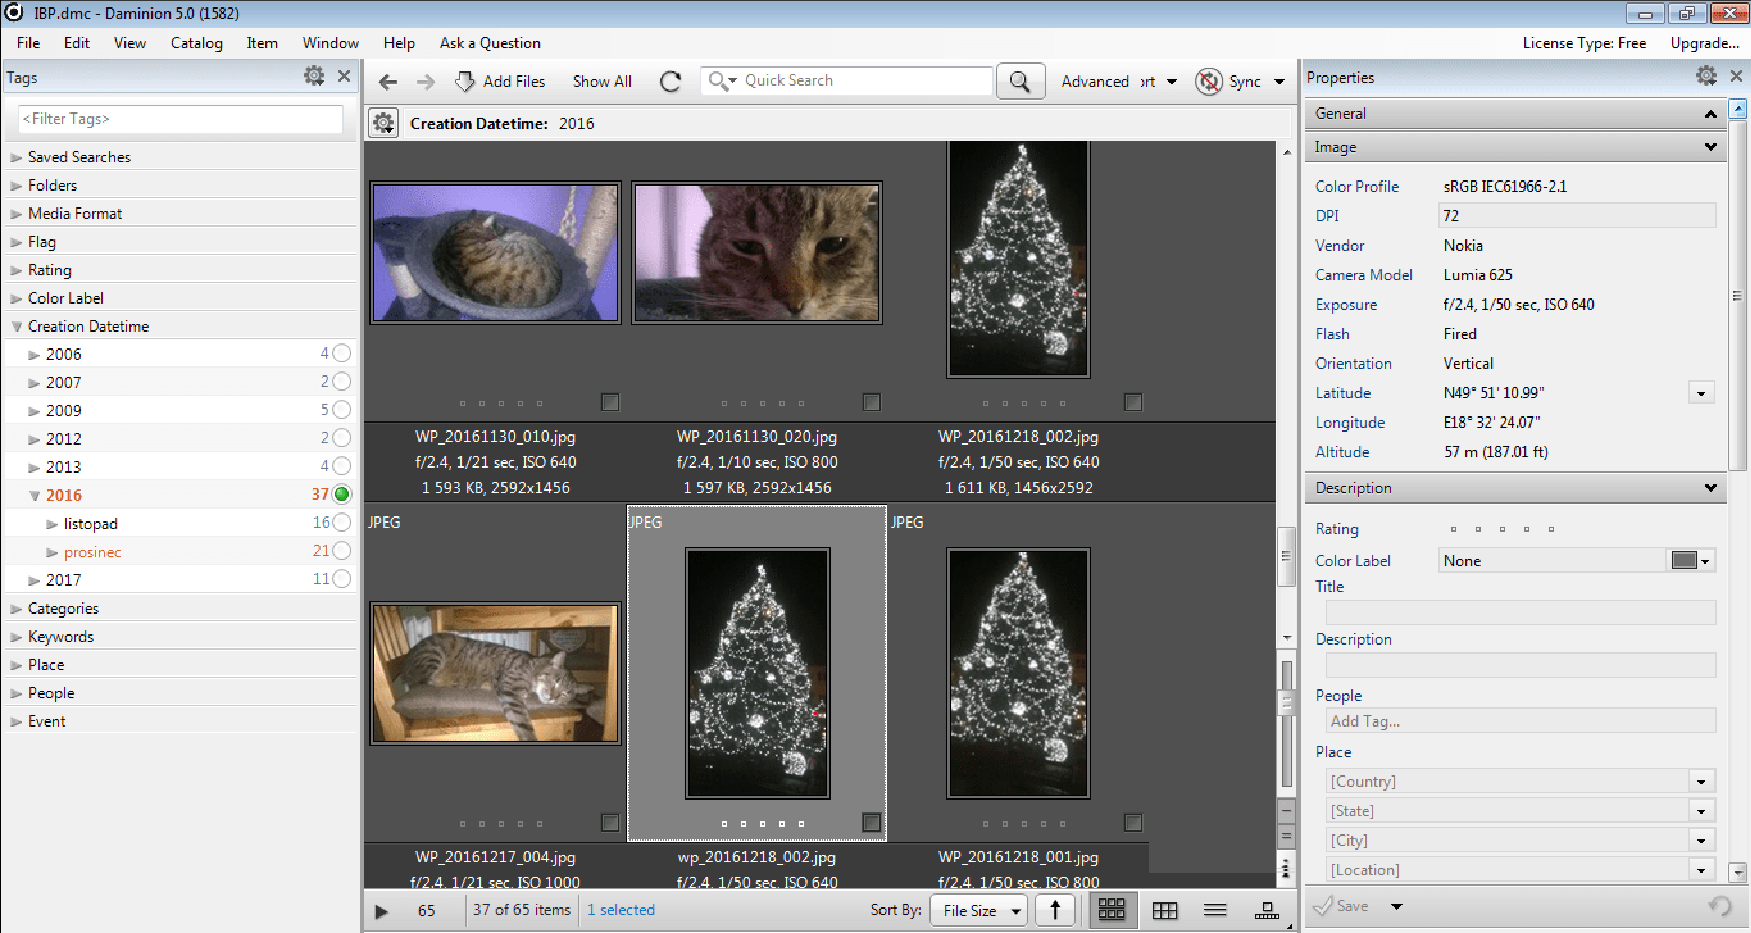
\includegraphics{obrazky-figures/Daminion.pdf}}
\caption{Hlavní okno programu Daminion}
\label{daminion_ob}
\end{center}
\end{figure}

Program Daminion od firmy Daminion Software \cite{Daminion} je taktéž určený pro správu digitálního obsahu počítače. Od ostatních se liší tím, že uživatel si může vytvořit vlastní sever, na který se bude nahrávat zpracovaný obsah a~následně s~ním může pracovat více uživatelů najednou. Je hlavně určený pro malé týmy uživatelů. Na obrázku \ref{daminion_ob} lze vidět okno aplikace s~již importovanými fotografiemi.

Práce s~tímto programem začíná vytvořením katalogu a~importováním požadovaných fotografií, přičemž lze fotografie nakopírovat přímo do vybrané složky a~smazat z~originálu nebo pouze importovat a~fyzicky ponechat na místě. Již při importu lze editovat Exif metadata a~případně rozdělit do kategorií podle jména adresářů (program vyhledává fotografie i~v~podadresářích).

Na levé straně program se nachází panel s~pomocí něhož, lze s~jednotlivými tagy  třídit zobrazené fotografie, na obrázku \ref{daminion_ob} lze vidět zaznačené fotografie, které mají datum vytvoření v~roce 2016. Tagy v~této sekci lze kombinovat, ale pomocí pokročilého vyhledávání v~menu rychlého přístupu (menu nad zobrazovací oblastí pro fotografie) je možné vyhledávat podle složitějších kombinací včetně i~vyhledávání pomocí Exif metadat.

Panel na pravé straně, který lze vidět na obrázku \ref{daminion_ob}, se zobrazí vyvoláním akce na zobrazení vlastností fotografie. Zobrazují se zde obecné informace o~souboru jako: jméno, cesta ke souboru, velikost souboru, tak i~Exif metadata a~mnohem více. Většina těchto dat lze modifikovat, je možné přidávat i~další dodatečné informace o~autorovi, klíčová slova nebo popisy. V~tomto panelu program nabízí zajímavou funkcionalitu\,-–\,při kliknutí na hodnotu nějaké vlastnosti se zobrazí fotografie, které v~dané hodnotě mají tu samou hodnotu.

Stejně jako Phototheca, tak i~Daminion umí vyhledat duplikáty (tato funkce bude popsána v~následující části kapitoly) a~podobně jako předcházející programy, tak i~tento je pouze správcem souborů a~neumožňuje grafické upravování digitálních fotografií. Také na rozdíl od výše představených programů tento neumí vytvářet tak zvaná chytrá alba, kdy se fotografie automaticky podle určitých kritérií roztřídí nebo vloží do alb. Určené skupiny fotografií umožňuje pouze zobrazit, ačkoliv po zaznačení zobrazených obrázku je umožňuje exportovat mimo program do daných adresářů a tím defacto vytvořit skupiny.

\section{Programy pro vyhledávaní duplikátu}
V~této části budou popsány 3~programy, které pomáhají vyhledat duplicitní soubory/fotografie. Duplicitní fotografie lze vyhledat mnohými způsoby, nejzákladnější vyhledávají pouze ty obrázky, které mají stejný název, další používají shodu v~Exif metadatech a~ty pokročilé kontrolují celá obrazová data. Co se týče poslední kategorie, tak v~tomto případě může takovéto prohledání najít i~fotografie, které se od sebe liší pouze v~maličkostech a~tím detekovat mnohačetné obrázky stejného objektu.

\subsection*{Phototheca}

Jak již bylo zmíněno dříve, tento program, kromě správy fotografií, umožňuje vyhledat i~jejích duplikáty. Na obrázku \ref{photo_dupl} lze vidět již vyhledané duplikáty. Program je vyhledává automaticky při importování fotografií. Zobrazit je lze stiskem tlačítka na levém panelu. 

\begin{figure}[h]
\begin{center}
\scalebox{0.49}{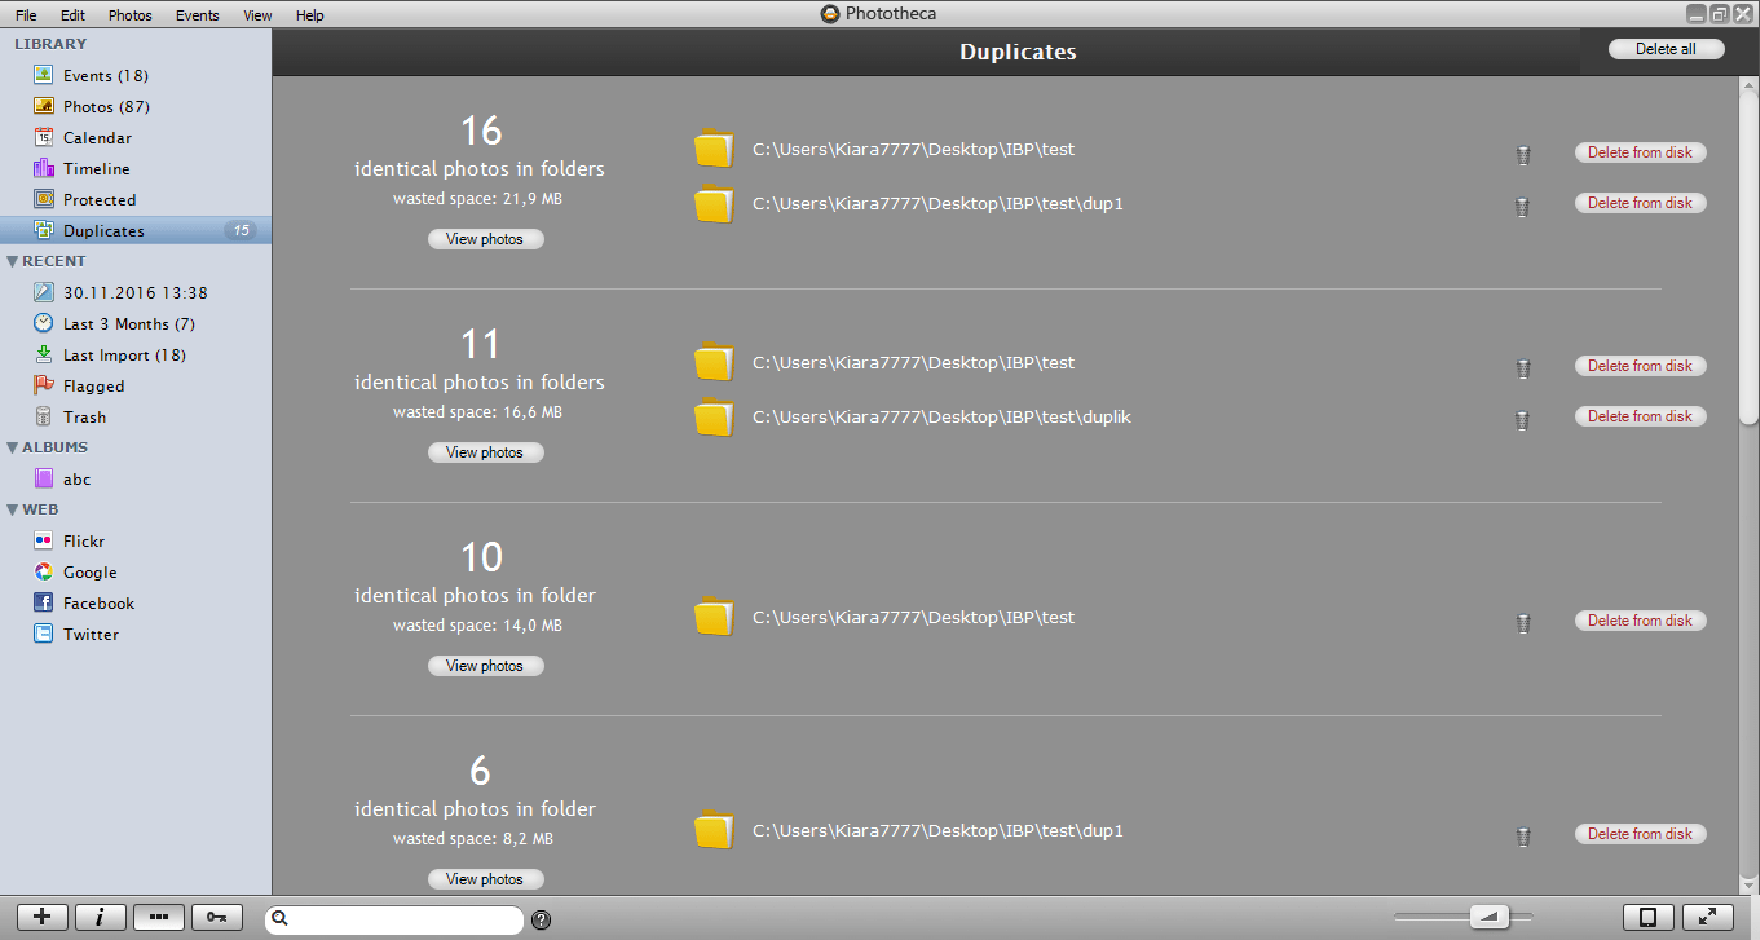
\includegraphics{obrazky-figures/Phototheca2Dupl.pdf}}
\caption{Vyhledané duplikáty v~programu Phototheca}
\label{photo_dupl}
\end{center}
\end{figure}

Nalezené fotografie mají podobu seznamu, při čemž při stisku \textit{View photos} se zobrazí miniatury obrázků, které jsou považovány za duplicitní. Fotografie se mohou smazat v~programu (při čemž se pouze odstraní jejích náhledy z~programu, skutečného souboru na disku se to nedotkne) nebo si lze vynutit odstranění z~disku. Při zvolení možnosti \textit{Delete all} nacházející se v~pravém horním roku programu, se odstraní miniatury všech duplicit kromě první fotografie, která se našla a~která je automaticky považována za originál.

Ačkoliv tvůrci programu nikde neuvádějí, jakým způsobem detekují duplikáty, lze uvažovat, že program využívá kombinaci Exif metadat a~obrazových dat, když nalezené duplicity nemají stejné názvy souborů a~v~případě, že daná fotografie má odstraněna metadata, tak i~tak je zahrnuta do duplikátů. Zajímavé ovšem je, že pokud se z~dat fotografie vyextrahuje preview (také známé jako thumbnail), tak ho Phototheca nerozezná jako duplikát k~originálu.

\subsection*{Daminion}

\begin{figure}[h!]
\begin{center}
\scalebox{0.49}{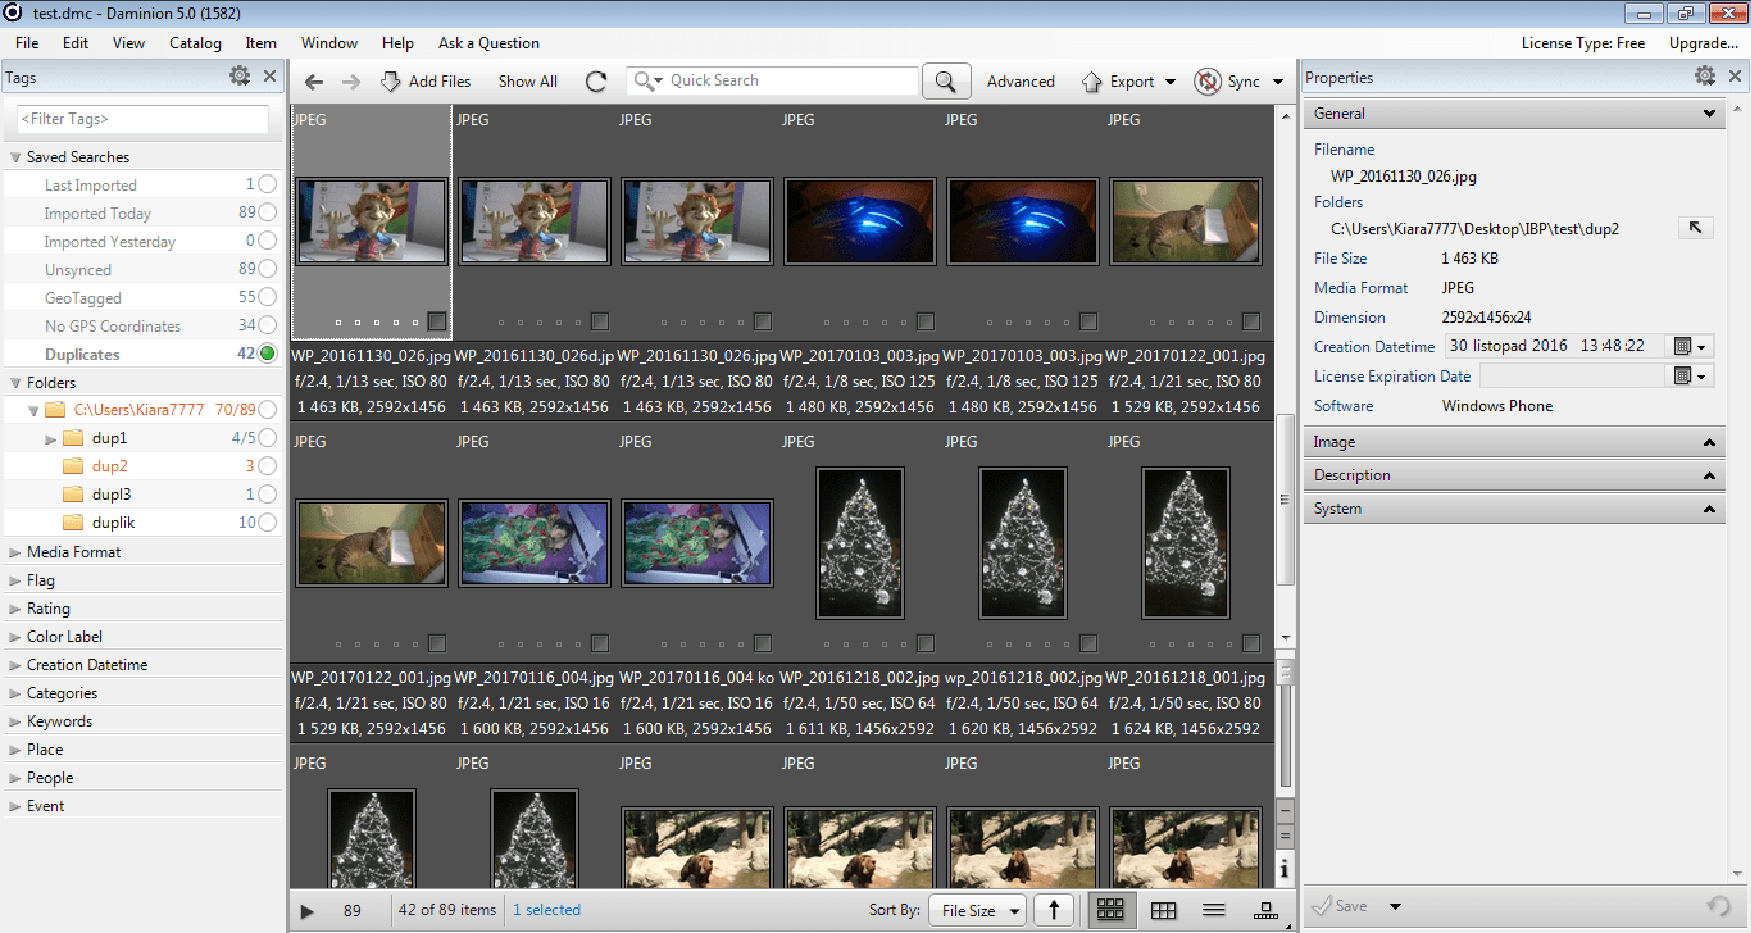
\includegraphics{obrazky-figures/daminion_dupl.pdf}}
\caption{Vyhledané duplikáty v~programu Daminion}
\label{dami_dupl}
\end{center}
\end{figure}

Také již dříve zmíněný program Daminion umí vyhledávat duplikáty. Obrázek \ref{dami_dupl} představuje již vyhledané duplikáty. Podobně jako Phototheca i~tady se vyhledají automaticky při importu fotografií. Je možné je zobrazit z~hlavního menu programu nebo z~levého bočního panelu, kde se, jak již bylo zmíněno dříve, může ovlivnit jaké kritéria musí fotografie splnit, aby se zobrazila.


Nalezené duplikáty se zobrazí všechny najednou a~nezáleží na jejích rozmístění v~adresářích. Danou fotografii pak lze smazat z~katalogu programu (skutečný soubor na disku se nesmaže) nebo se může odstranit jak z~katalogu, tak i~přesunout do koše. Při kliknutí na fotografii se také v~druhé rozkliknuté kategorii na levém panelu (viz. obrázek \ref{dami_dupl}) zaznačí adresář ve kterém se duplikát nachází, toto chování může pomoct detekovat duplicitní adresáře, takže se nemusí mazat fotografie jedna po druhé, ale rovnou celá složka s~nimi.

Duplikáty v~tomto programu se v~dřívějších verzích vyhledávaly na základě metadat. Dnešní verze dle webových stránek a fóra vývojářů \cite{Daminion} využívají obrazová data, ale v~případě, že duplicitní fotografie má jinou orientaci než originál, tak nebude považována za duplikát.

\subsection*{Easy Duplicate Finder}

Easy Duplicate Finder \cite{EDF} je program umožňující vyhledávání duplikátů mnoha formátů. Dokáže zpracovat dokumenty, e-maily, textové nebo hudební soubory, a~také právě digitální fotografie.
Na obrázku \ref{edf_dupl} lze vidět třetí a~zároveň poslední krok v~tomto nástroji\,-–\,zobrazení vyhledaných duplikátů.

\begin{figure}[h]
\begin{center}
\scalebox{0.49}{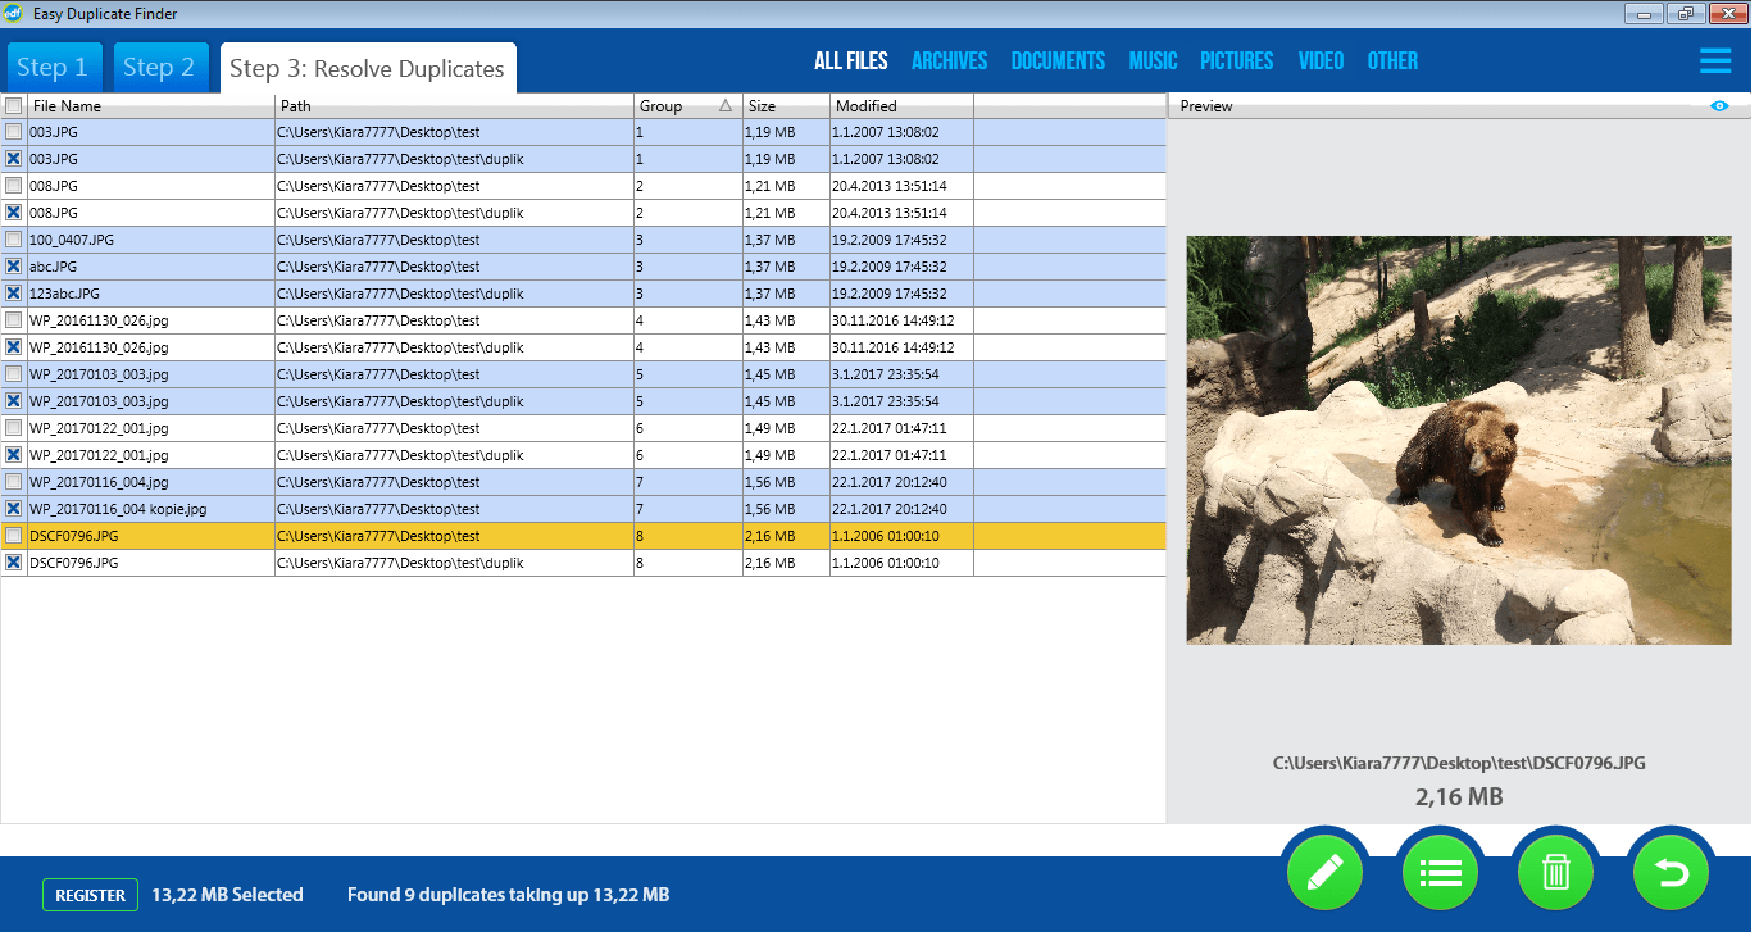
\includegraphics{obrazky-figures/edf.pdf}}
\caption{Vyhledané duplikáty v~programu Easy Duplicate Finder}
\label{edf_dupl}
\end{center}
\end{figure}

Prvním krokem je výběr adresářů kde se mají duplikáty vyhledávat a~určení s~jakým typem souborů se bude pracovat. Následuje skenování a~zobrazení shrnujících informací o~tom kolik se zpracovalo souborů, kolik bylo duplikátu a~kolik se uvolní místa na disku, v~případě, že se duplikáty odstraní. A~jak již bylo zmíněno, ve třetím kroku je lze zobrazit. Nalezené fotografie mají podobu seznamu, ve kterém se při kliknutí na danou položku zobrazí náhled na fotografii. Následně lze duplikáty odstranit, přesunout do jiné složky nebo odstranit adresář, ve kterém se fotografie nachází, z~programu nebo z~disku.

Ačkoliv vývojáři opět neuvádějí, jakým způsobem rozeznávají duplikáty, lze předpokládat, že k~tomu využívají alespoň nějaké informace z~Exif metadat, když rozezná i~soubory, které mají rozdílné názvy. Ovšem v~případě, že dané duplicitě byla odstraněna metadata, tak ji program nerozezná. 

\chapter{Návrh funkcí pro správu skupin fotografií}
\label{Nvr}

V~této kapitole se zhodnocuje dosavadní stav řešení problému rozdělování fotografií do skupina a~hledaní jejích duplicit, přičemž se opírá o~dříve představené programy. Následně se zde popisuje návrh funkčnosti programu, který se má vytvořit.

\section{Zhodnocení dosavadního stavu}

V~předcházejí kapitole byly představeny některé programy, které jsou schopné rozdělit fotografie do skupin nebo je alespoň zobrazit podle určitých kritérií. Všechny tyto programy jsou komplexní a~umožňují velké množství funkcí pro správu fotografií. Pro některé, hlavně pro méně zkušené hráče, toto může být překážkou, když hledají pouze jednu funkci a~nechtějí se dopodrobna seznamovat s~celým program. Většina z~těchto nástrojů vyžaduje, aby se fotografie nejdříve naimportovaly do programu, a~až poté je umožněno s~nimi pracovat. Všechny umožňují prohlížet Exif metadata, některé položky z~metadat lze mazat nebo editovat, taktéž dovolují přidávat jména autorů, komentáře nebo popis fotografie. Podpora jednotlivých tagů metadat se v~programech liší. Fotografie v~těchto programech lze i~hodnotit, ale tato funkce slouží pouze pro potřeby v~daném programu. Představné programy umožňují zobrazovat nebo tvořit skupiny, ale pouze Phototheca je schopna danou skupinu vytvořit automaticky mimo program, v~dalších programech je musí uživatel vytvořit sám přes zaznačení jednotlivých fotografií a~stisk tlačítka nebo je ručně přesunout do složky.

Co se týče programů pro vyhledávání duplicit, tak ty ve většině případů využívají Exif metadata a~ty pokročilejší vyhledávají na základě podobnosti obrazový dat. Jsou zobrazovány buď v~podobě seznamu nebo jako náhledy na fotografie. To, jaké jsou duplicitní lze jednoduše rozpoznat, když jsou zobrazované jako jedna skupina nebo jsou v~seznamu vedle sebe. Představené nástroje je umožňují smazat všechny najednou přičemž ponechají první, kterou nalezli a~kterou považují na originál, nebo je lze smazat všechny zaznačené, případně jednu po druhé. Při odstraňování se uživatel může rozhodnout, zda je pouze vymaže z~indexu programu nebo také z~disku. Žádný z~představených programů ovšem nedokáže zobrazit v~jaké skupině se duplikát nachází, případně zda jsou přítomné nějaké duplicitní skupiny.

V~následující tabulce \ref{prehled_prog} lze najít souhrn informací o~funkcích programů představených v~kapitole \ref{Ex_prg}.

\begin{table}[]
\centering
\begin{tabular}{|c|c|c|c|c|}
\hline
                                                                & Import & Skupiny & Duplicity & Metadata \\ \hline
Adobe Bridge CC                                                 &        & \ding{51} &           &\ding{51} \\ \hline
Phototheca                                                      &\ding{51} &\ding{51} &\ding{51} & \ding{51}\\ \hline
Daminion                                                        &\ding{51} &\ding{51} &\ding{51} &          \\ \hline
Easy Duplicate Finder											&        &         &\ding{51}&          \\ \hline
\end{tabular}
\caption{Přehled funkčnosti programů}
\label{prehled_prog}
\end{table}

\section{Návrh funkcí}

Na základě analýzy dosavadního stavu řešené problematiky, zadání práce a~osobních preferencí jsem navrhla funkce, které by měl program splňovat. Vytvořená aplikace by měla fungovat na systému Windows a měla by umožňovat:

\begin{itemize}
\item Zobrazovat fotografie a~jejích Exif metadata
\item Rozdělovat fotografie do skupin
\item Ukládat skupiny na disk
\item Vyhledávat duplikáty vevnitř skupin
\item Vyhledávat duplicitní skupiny
\item Mazat duplikáty
\end{itemize}

Uživateli by mělo být umožněno zobrazovat načtené fotografie a~některá jejích Exif metadata. Pro potřeby programu jsem usoudila že by bylo vhodné zobrazovat: jméno fotografie, velikost souboru v~megabytech, datum vytvoření a~GPS souřadnice.

Aplikace by měla rozdělovat fotografie do skupin pomoci datumu vytvoření nebo GPS souřadnic místa vytvoření, přičemž uživatel bude moct zadat podle jakého kritéria se má rozdělovat. Vytvořené skupiny by měly jít smazat jak z~programu, tak z~pevné disku (společně se skupinami by se měly smazat i~fotografie v~nich obsažené). Taktéž by mělo být možné, aby se skupiny následně vytvořily jako adresáře a~do nich se přenesly odpovídající fotografie.

Pro urychlení programu by se měly duplikáty vyhledávat pomocí Exif metadat. Pokud by se měla použít obrazová data, mohlo by to prohledávání výrazně prodloužit, když velikost těchto dat mnohonásobně převyšuje velikost několika hodnot z~metadat. V~případě vnitřních duplikátu, tak ty by se měly zobrazovat v~jaké skupině se nachází. Duplicitní skupiny by se mohly zobrazovat společně s~informacemi k~jaké skupině jsou duplicitní, dále by také mělo zobrazovat jaké fotografie v~obou skupinách jsou k~sobě duplicitní. Uživatel následně bude moct rozhodnout, kterou skupinu odstraní.


\chapter{Realizace a~implementace}
\label{Real}

Na začátku této kapitoly se popisuje návrh rozhraní aplikace a~také způsob jakým se otestuje její funkčnost. Dále pak lze najít popis výsledného programu a~způsob jeho implementace.  Na konci se pak nachází průběh a~výsledky testování.

\section{Návrh uživatelského rozhraní}
Na obrázku \ref{navrh_hl} lze vidět návrh rozložení prvků v~uživatelském rozhraní.

\begin{figure}[ht]
\begin{center}
\scalebox{0.7}{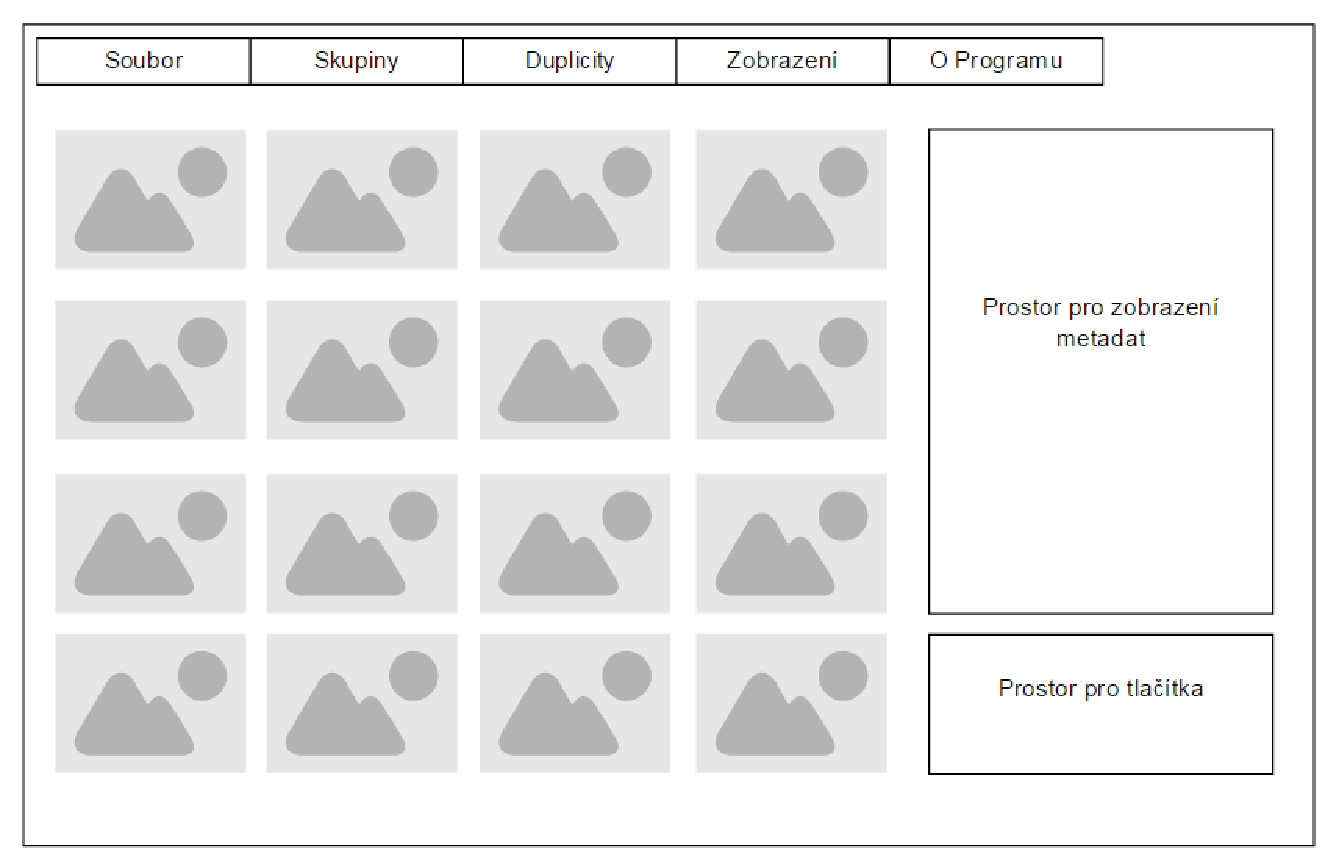
\includegraphics{obrazky-figures/skup.pdf}}
\caption{Návrh rozhraní pro zobrazování fotografií, skupin a~duplikátů}
\label{navrh_hl}
\end{center}
\end{figure}

Okno programu je při prohlížení neroztříděných fotografií, skupin a~duplikátu rozdělené na dvě části. Na levé straně se nacházejí náhledy na fotografie a~v~pravé části lze nalézt zobrazená jednotlivá metadata. Pod částí s~metadaty je na pravé straně nacházejí také tlačítka pomoci, kterých může uživatel skupinu uložit na pevný disk nebo zaznačený objekt odstranit. Program se bude ovládat pomocí menu aplikace. \texttt{Soubor} umožní skenovat fotografie, exportovat výsledné rozložení a~ukončit program, možnost \texttt{Skupiny} otevře dialogové okno pro nastavení vyhledávání skupin a \texttt{Duplicity} umožní vyhledat duplikáty vevnitř i~mezi skupinami. V~\texttt{Zobrazení} se bude moct přepínat mezi jednotlivými okny a~v~\texttt{O~Programu} se uživatel dozví základní informace o~aplikaci.

Rozložení prvků v~aplikaci v~době zobrazování duplicitních skupin si lze prohlédnout na obrázku \ref{navrh_dupl}. 


\begin{figure}[ht]
\begin{center}
\scalebox{0.7}{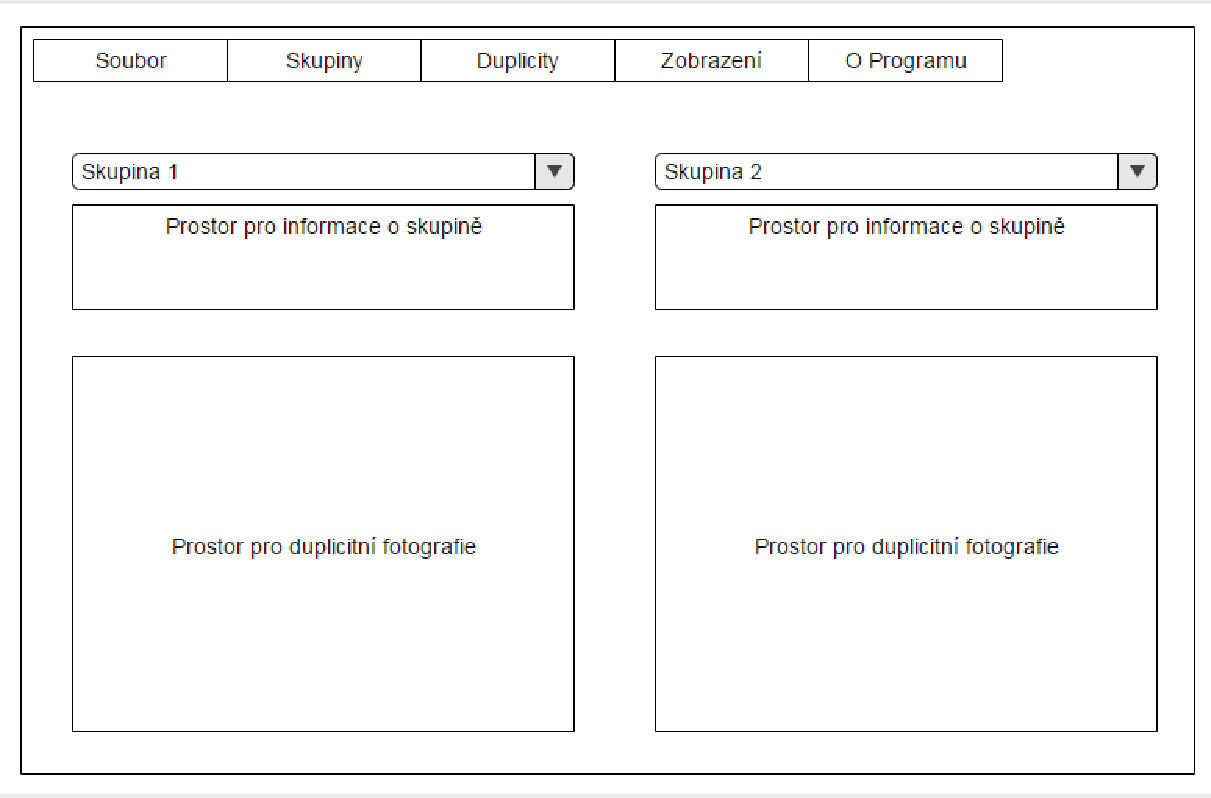
\includegraphics{obrazky-figures/duplSkup.pdf}}
\caption{Návrh rozhraní pro zobrazování duplicitních skupin}
\label{navrh_dupl}
\end{center}
\end{figure}

V~kombinovaných seznamech se nacházejí duplicitní skupiny, přičemž druhý sloupec reaguje na to, co je zobrazováno v~prvním (ve druhém sloupci se zobrazují skupiny, které jsou duplicitní ke skupině v~prvním sloupci). V~informacích o~skupině se zobrazuje, kolik má daná skupina fotografií celkově a~kolik duplikátů vzhledem ke skupině ve vedlejším sloupci. V~prostoru pro duplicitní fotografie se pak zobrazují náhledy fotografií, které jsou duplicitní k~druhé skupině.

\section{Návrh otestování funkčnosti}

Testování bude probíhat ve dvou fázích. První fáze se bude skládat z~několika různých testů, které mají ověřit, zda program správně rozdělí fotografie do skupin podle zadané kategorie a~také zda správně určil duplikáty. Přitom se také ověří, jak dlouho bude počítači trvat jednotlivé úkoly vykonat. 
Druhá fáze se zaměří na uživatele a~jeho práci s~programem. Uživatel bude plnit jednotlivé úkoly, přičemž se bude pozorovat, jak je plní a~taktéž se bude měřit čas, jak dlouho mu daný úkol trvalo splnit. Následně se s~uživatelem provede rozhovor, ve kterém se probere, jak se mu z~aplikací pracovalo, zda mu přišla intuitivní, co by změnil a jestli by program používal i~v~budoucnosti.

\section{Vzhled aplikace a~popis její funkcí}
Na obrázku \ref{VSE_P} lze vidět jedno z~oken výsledné aplikace. Jak již bylo v~částí Návrh uživatelského rozhraní zmíněno, okno je rozděleno na 2 části. Na levé straně se zobrazují náhledy na fotografie na pravé straně se při kliknutí na náhled zobrazí informace o~dané fotografii. Program umožňuje zobrazovat čtyři stavy\,–-\,nerozdělené fotografie, skupiny, duplikáty fotografií vevnitř skupin a~duplicitní skupiny. Přepínání mezi jednotlivými stavy lze uskutečnit v~menu programu pod záložkou \texttt{ZOBRAZENO}. Z~menu se také ovládá celá aplikace. Ještě předtím, než je možné s~programem pracovat, tak se musí jednotlivé fotografie do něho naimportovat.

\begin{figure}[h]
\begin{center}
\scalebox{0.5}{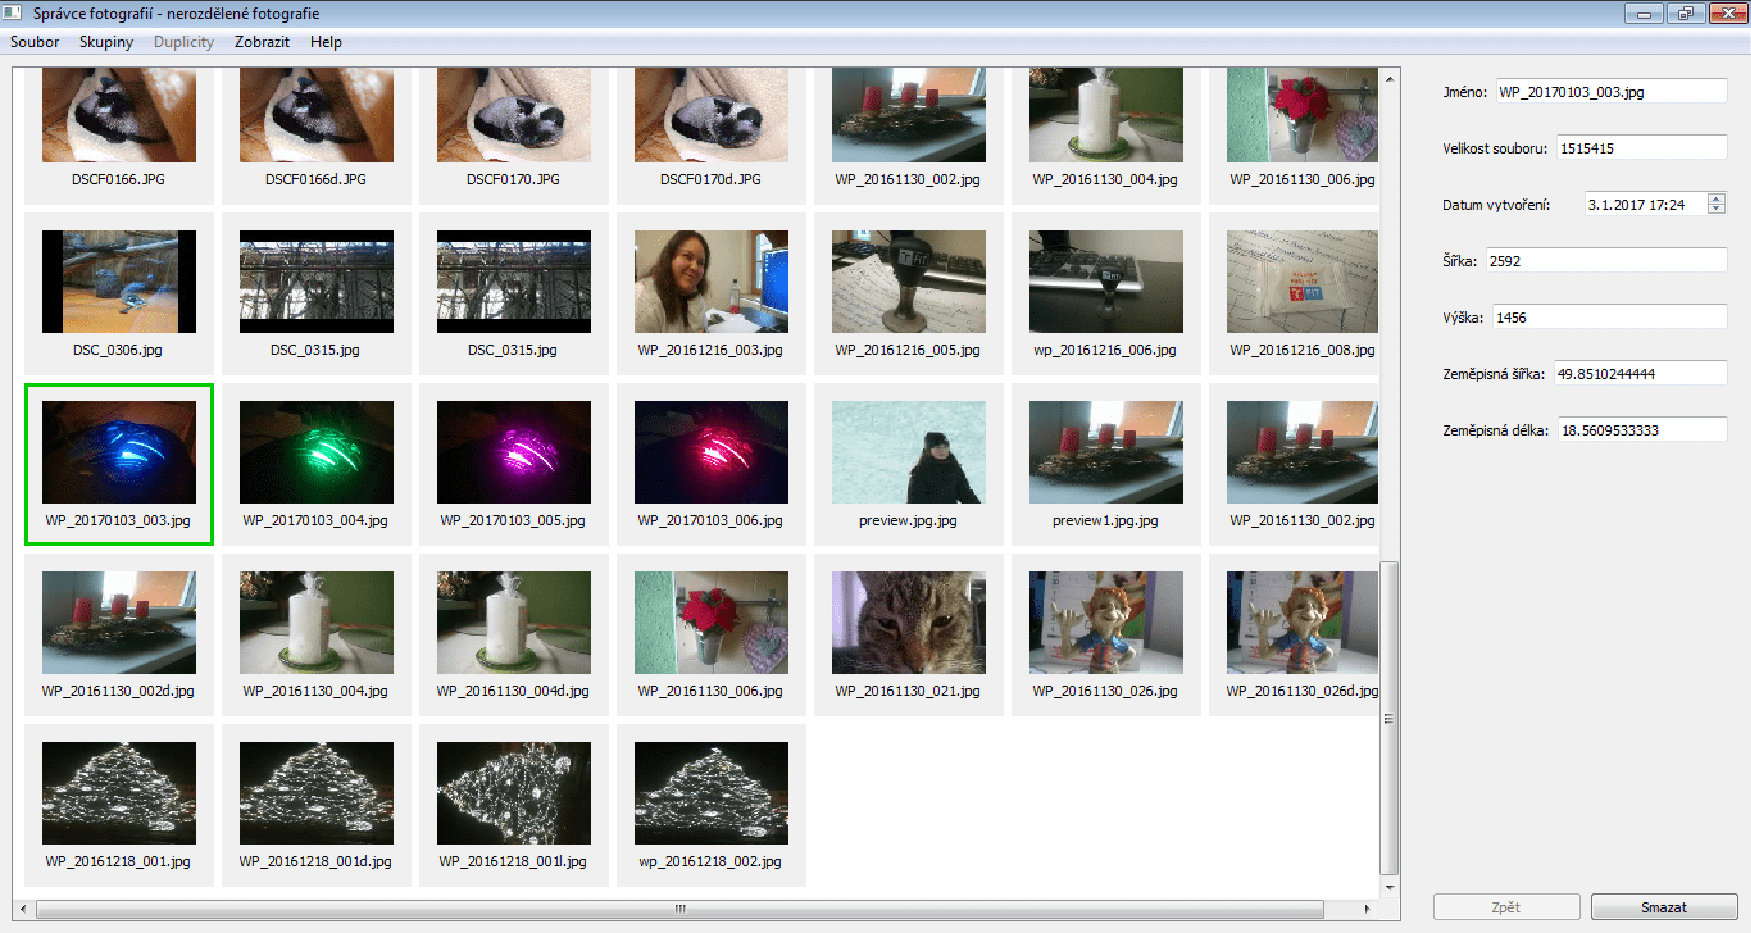
\includegraphics{obrazky-figures/VSE_P.pdf}}
\caption{Zobrazení nerozdělených fotografií}
\label{VSE_P}
\end{center}
\end{figure}

\subsection*{Načítání fotografií}

Ještě před tím, než se může s~aplikací pracovat, tak se musí jednotlivé fotografie načíst a~získat z~nich potřebná Exif metadata. Pro potřeby programu se získávají tyto data: datum vytvoření, šířka a~výška v~pixelech a~GPS souřadnice místa vytvoření. Další data (jméno a~velikost souboru fotografie), lze pak získat z~informací o~souboru a~není potřeba je vyhledávat v~metadatech.

Pro získání adresáře, ze kterého se mají fotografie zpracovat, se používá třída QFileDialog. V~tomto adresáři se následně skenují fotografie, které mají JPEG formát (mají koncovku souboru JPG nebo jpg). Prohledávají se také podadresáře dané složky. Jednotlivé informace se pak automaticky ukládají do textového souboru, takže uživatel může po načtení dat program vypnout bez případné ztráty dat.

Extrakce metadat ovšem může trvat delší dobu, a~proto se při načítání fotografií zobrazuje dialog, který informuje uživatele o~tom, že program nezamrzl a že pokračuje ve zpracovávání a~také mu umožňuje vyhledávání stornovat.

K~získávání metadat je také svázána jedna optimalizace vyhledávání a~ukládání. V~případě, že už jednou byly fotografie skenovány tak se u~právě načítaných dat kontroluje pouze celé jméno daného souboru a~jeho velikost v~bajtech. Díky tomu odpadne potřeba danou fotografii otevírat a~extrahovat z~ní data a~tím se doba pro načítání mnohonásobně zkrátí.


\subsection*{Dvojí zobrazování}

Pro urychlení práce s~programem se fotografie ve výchozím stavu zobrazují jako seznam položek. Díky tomu se může vynechat krok s~načítáním náhledů fotografií (tato činnost, je vysvětlena v~následující části). Na obrázku \ref{VSE_S}, lze vidět zobrazení fotografií, které koresponduje se zobrazením na obrázku \ref{VSE_P}. Přepínání mezi jednotlivými styly zobrazování lze uskutečnit v~menu programu pod záložkou \texttt{ZOBRAZENO}.

\begin{figure}[h]
\begin{center}
\scalebox{0.5}{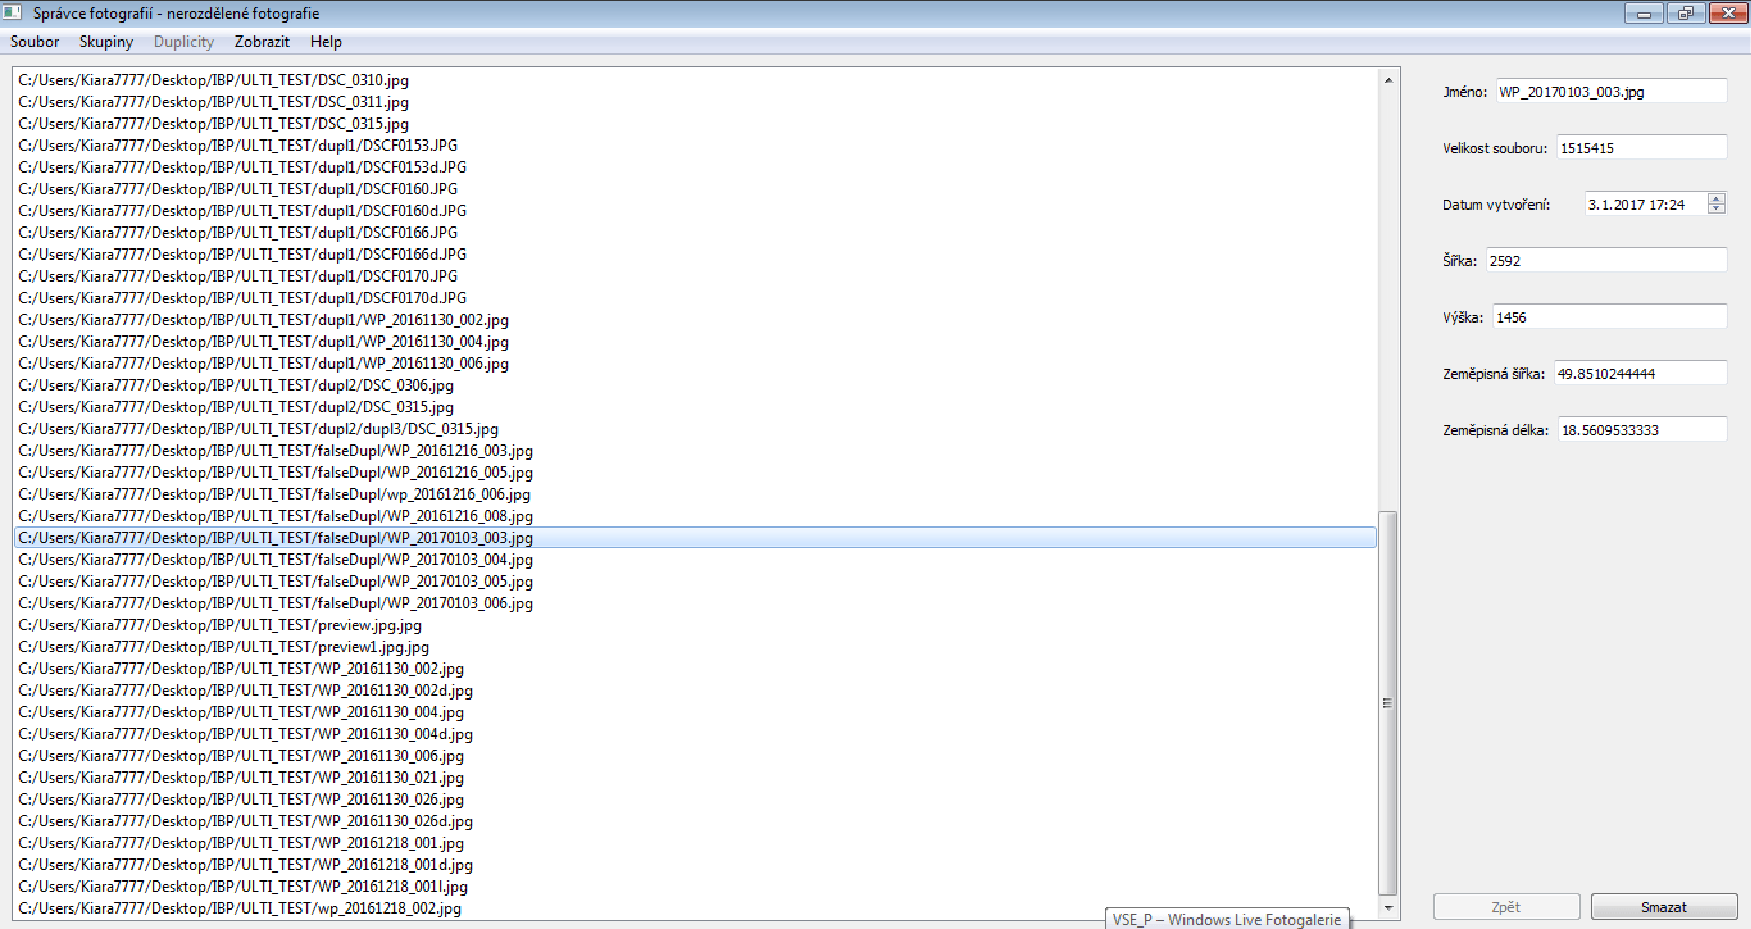
\includegraphics{obrazky-figures/VSE_S.pdf}}
\caption{Zobrazení nerozdělených fotografií v~seznamu, koresponduje s~\ref{VSE_P}}
\label{VSE_S}
\end{center}
\end{figure}

\subsection*{Načítání náhledů}

Jak již bylo zmíněno, výchozím chováním programu je zobrazovat fotografie jako seznam. Při zvolení zobrazování pomocí náhledů na fotografie se zavolá potřebná funkce, která pomocí Exif2 knihovny, získá z~obrázků potřebná data.

Náhledy na fotografie se ukládají při jejím vzniku do Exif metadat. Někdy se ovšem může stát, že náhled v~metadatech není obsažen\,-–\,ať už ukládání nepodporuje digitální fotoaparát, nebo samotná fotografie neobsahuje Exif metadata. Pokud taká situace nastane, tak se načítá celý obraz fotografie. Výsledná miniatura se následně zmenší do požadované velikosti a~zobrazí do mřížkového rozložení, které lze vidět na obrázku \ref{VSE_P}. Nevýhodou tohoto chování může být, že ačkoli mají miniatury stejnou velikost, tak při bližším pohledu na náhled lze vidět nepřirozené zmenšení nebo rozšíření obrazu \ref{VSE_P_NEPR}.

\begin{figure}[h]
\begin{center}
\scalebox{1}{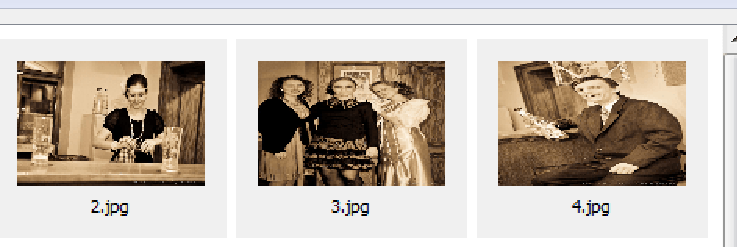
\includegraphics{obrazky-figures/fotoNepr.pdf}}
\caption{Dvě nepřirozeně zmenšené fotografie}
\label{VSE_P_NEPR}
\end{center}
\end{figure}

Podobně jako u~samotné extrakce informací z~fotografie, tak i~tady se z~důvodu možné nezanedbatelně dlouhé doby načítání obrazu zobrazuje dialog, který uživatele informuje o~stavu dané operace a~také mu umožňuje operaci přerušit.

\subsection*{Rozdělování do skupin}

Jak již bylo zmíněno, program se ovládá pomocí menu hlavního okna. Pod záložkou \texttt{SKUPINY} lze vyvolat dialogové okno \ref{Dialog_Skupiny} pomocí kterého se může určit podle jakého kritéria se mají fotografie rozdělit. 
V~současné době se rozděluje buď pomocí datumu vytvoření nebo pomocí GPS souřadnic. Druhý řádek v~dialogu umožňuje určovat v~jakém časovém intervalu se musí zkoumaná fotografie nacházet, aby se mohla stát členem dané skupiny, při čemž tento interval ovlivňuje poslední fotografie, která byla do skupiny přidána. Předcházející věta platí pro rozdělování podle datumu vytvoření, pro rozdělování pomocí GPS je tímto intervalem vzdálenost.

\begin{figure}[h]
\begin{center}
\scalebox{1}{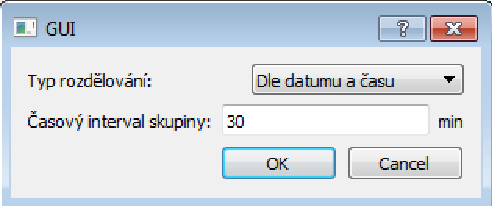
\includegraphics{obrazky-figures/SK_dia.pdf}}
\caption{Dialog pro rozdělení do skupin}
\label{Dialog_Skupiny}
\end{center}
\end{figure}

Vzdálenost u~rozdělování pomocí GPS souřadnic se počítá pomocí Haversinovy formule \cite{Haversine}. Podle \cite{WHYHaversine} lze díky této metodě získat velmi přesné výsledky i~pro vzdálenosti v~hodnotách několika desítek metrů.

Jak již bylo řečeno, je možné, že daná fotografie nebude mít Exif metadata nebo jí potřebná data budou chybět (digitální fotoaparáty většinou nepodporují ukládání GPS souřadnic místa vytvoření do metadat fotografie). Proto se tyto obrázky automaticky ukládají do skupiny \texttt{Nezařazeno}. Fotografie, které nemají v~sobě GPS se do této skupiny ukládají pouze, při rozdělování pomocí GPS.

Zobrazení skupin v~programu je podobné jako zobrazování nerozdělených fotografií, při čemž dvojím kliknutím na skupinu se zobrazí fotografie k~ní přiřazené. Zpět na zobrazení skupin je tak možné pomocí tlačítka \texttt{Zpět} na pravé dolní straně programu.

\begin{figure}[h]
\begin{center}
\scalebox{0.7}{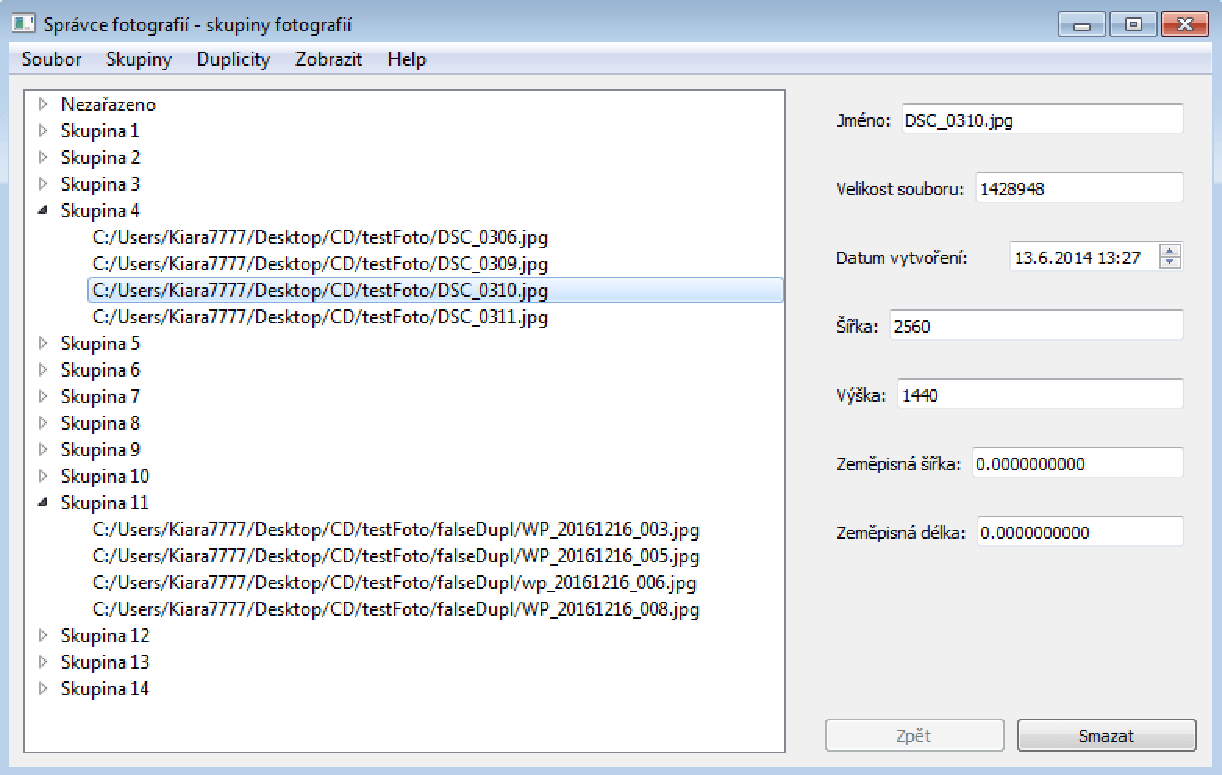
\includegraphics{obrazky-figures/SK_S.pdf}}
\caption{Zobrazení skupin v~podobě seznamu}
\label{SK_S}
\end{center}
\end{figure}

\subsection*{Hledání duplikátů}
Duplikáty se mohou vyhledat pouze pokud fotografie již byly rozděleny do skupin. Program umožňuje vyhledat dva typy identických fotografií\,–-\,vnitřní ve skupinách anebo duplicitní skupiny. Pro každý typ se vytváří vlastní zobrazení v~hlavním okně aplikace. Vyhledávají se automaticky po zvolení požadovaného typu pod záložkou \texttt{DUPLIKÁTY} v~menu aplikace.

Duplicitní fotografie se detekují pomoci shody Exif metadat, z~načtených dat se pro tento účel využívají velikost souborů v~bytech, datum a~čas vytvoření, výška a~šířka fotografie v~pixelech. Fotografie jsou považovány za identické, pokud souhlasí všechny hodnoty z~daných dat. Pro porovnávání se nepoužívá jméno souboru dané fotografie, protože tento údaj lze velmi jednoduše změnit ať uživatelem při jejím zpracováním nebo programem, který se použil pro její import. Taktéž se nevyužívají GPS souřadnice, protože fotografie tento údaj nemusí obsahovat.

V~předcházející části této kapitoly bylo zmíněno, že fotografie, které nemají potřebná data (GPS souřadnice) nebo neobsahují Exif metadata se vkládají do skupiny \texttt{Nezařazeno}. Jelikož se tyto fotografie nemají, jak porovnat, tak se skupina \texttt{Nezařazeno} při hledání duplikátu vynechává.

Vnitřní duplikáty se v~módu náhledů na fotografie zobrazují podobně jako skupiny nebo nerozdělené fotografie. Jedinou změnou je, že v~okně aplikace budou obsaženy jenom skupiny, které tyto duplikáty obsahují. Při rozkliknutí skupiny, se zobrazí pouze identické fotografie, které se v~ní nacházejí. I~tady se uživatel následně může vrátit zpět na zobrazení skupin, které mají v~sobě duplikáty. V módu seznamu je to podobné, rozdílem je, že zobrazení obsahuje o~jednu úroveň více (lze vidět na obrázku \ref{DIN_S}). Na této úrovni se nachází fotografie, ke které se nalezl duplikát, ale jelikož byla v~seznamu první, tak se prohlásila za \uv{hlavní} a~z~toho důvodů se nachází o~úroveň výše.

\begin{figure}[h]
\begin{center}
\scalebox{0.7}{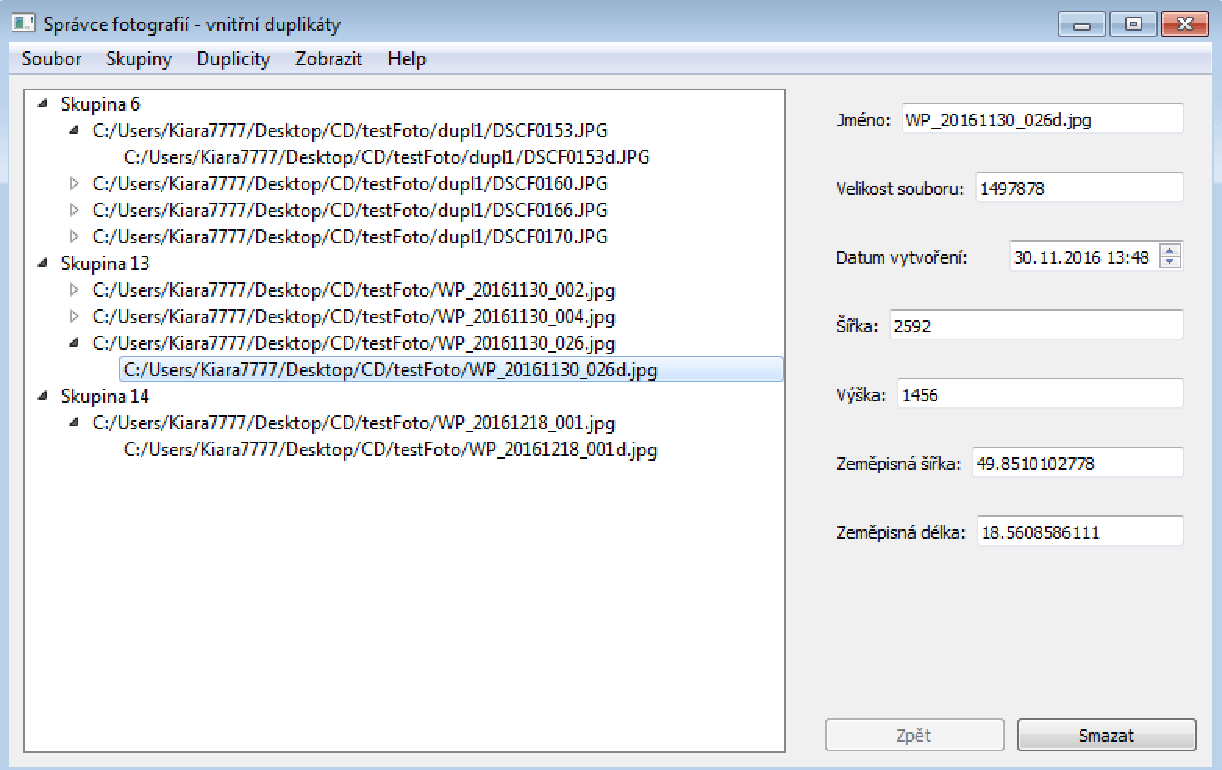
\includegraphics{obrazky-figures/DIN_S.pdf}}
\caption{Zobrazení vnitřních duplikátů ve skupinách v~podobě seznamu}
\label{DIN_S}
\end{center}
\end{figure}

Pro duplikáty skupin existuje odlišné okno než doposud (k~vidění na obrázku \ref{DSK_P}). Ve sloupci na pravé straně se zobrazují informace o~duplicitních skupinách ke skupinám nacházejících se v~levém sloupci. To, jaká dvojice skupin je zrovna na obrazovce se ovládá pomocí rozbalovacích seznamů. Pod každým se pak následné zobrazuje, kolik má daná skupina celkově fotografií a~kolik jich je duplicitních ke druhé skupině. Pod tím vším lze pak nalézt, které to jsou ať už v~podobě seznamu nebo jako jejích miniatury.

\begin{figure}[h]
\begin{center}
\scalebox{0.5}{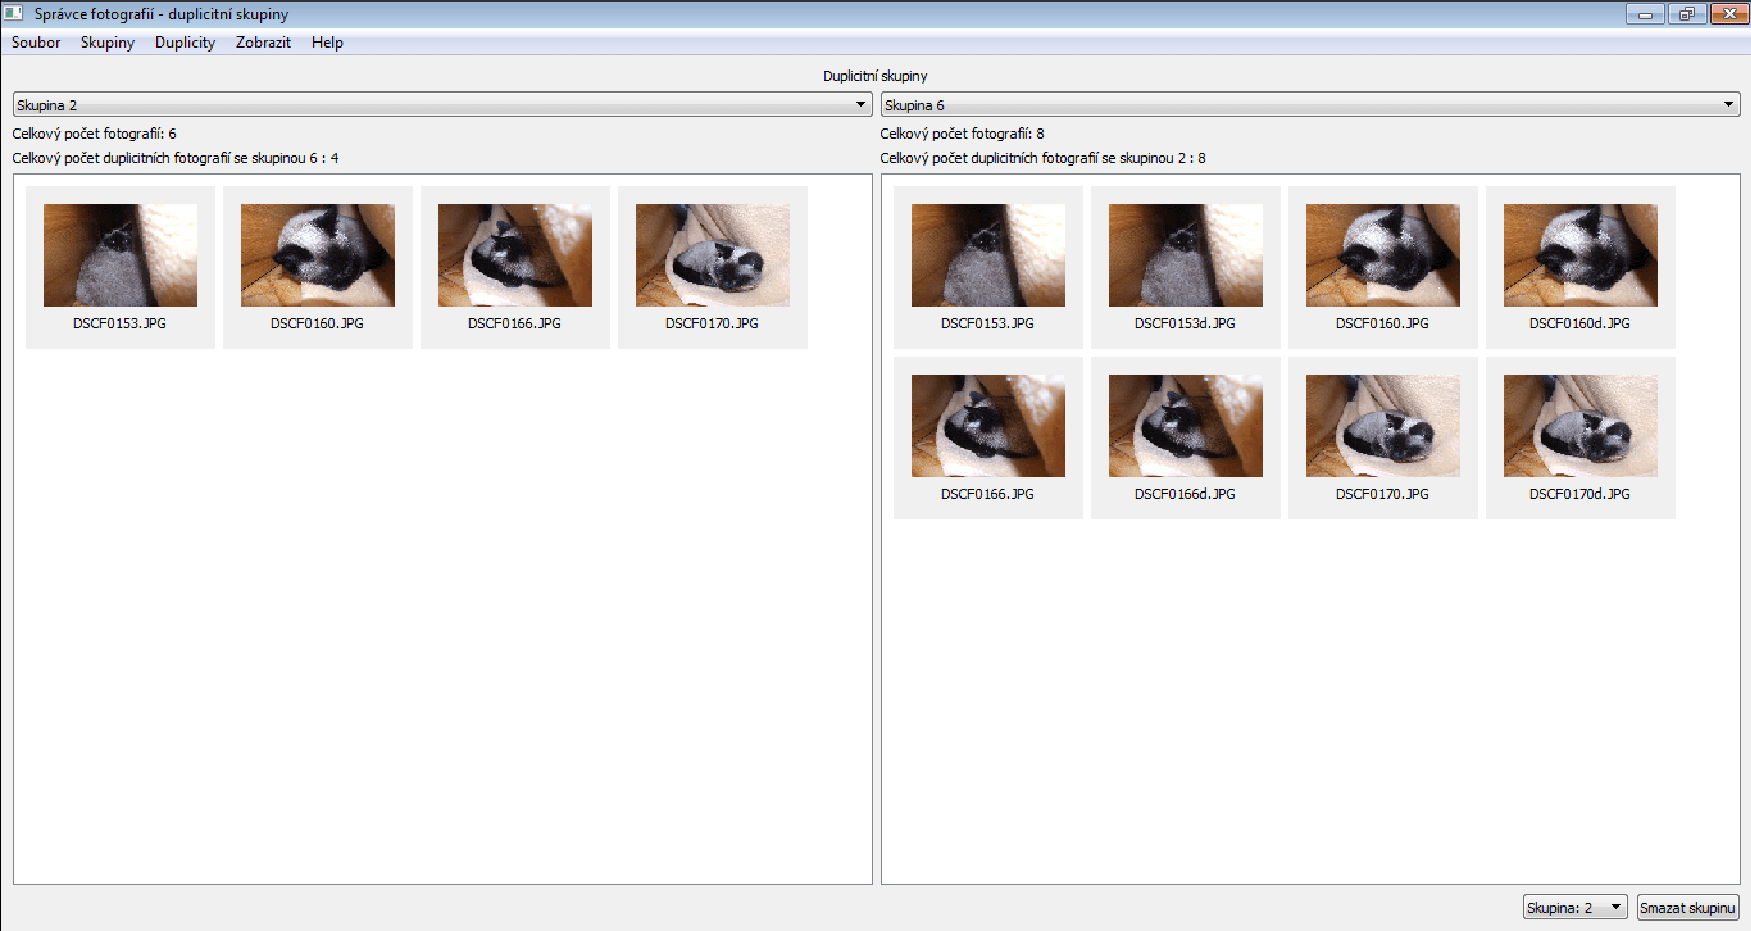
\includegraphics{obrazky-figures/DSK_P.pdf}}
\caption{Zobrazení duplicitních skupin v~podobě náhledů}
\label{DSK_P}
\end{center}
\end{figure}

\subsection*{Odstraňování fotografií}

V~každém stavu programu (zobrazení nerozdělených fotografií, skupin, vnitřních duplikátů nebo duplicitních skupin) je možné zahájit akci odstraňování. Je možné smazat neroztříděnou fotografii, fotografii ve skupině nebo samotnou skupinu. Nezáleží, v~jakém stavu aplikace se fotografie smaže, program bude udržovat struktury skupin a zobrazení všech stavů vždy aktuální.

Fotografii nebo skupinu, lze smazat jejím označením a~stisknutím tlačítka \texttt{Smazat}, které se nachází v~pravém dolním roku programu. Zaznačená fotografie se zvýrazní zeleným rámečkem, skupina se obarví rámečkem modrým. V~módu seznamu se pouze zvýrazní řádek, na které se daný záznam nachází.

Důležitým faktem je, že se odstraňují pouze záznamy vytvořené v~programu, skutečné soubory na místě uložení nejsou ovlivněny. Díky tomuto přístupu se nezatěžuje procesor a disk počítače, kteří by v~opačném případě museli každou fotografii nalézt a~smazat. Pokud uživatel chce, aby se výsledky přenesly i~na disk, musí veškerou svou práci s~programem uložit, o~čemž se píše v~následující částí.  

\subsection*{Export výsledného rozdělení}

Aplikace si pamatuje veškeré změny provedené s~fotografiemi (rozdělování, odstraňování). Změny se ovšem neukládají automaticky, ale pouze na pokyn uživatele. Toto uložení lze vyvolat pod záložkou \texttt{Program} a~\texttt{Exportovat fotografie}. Akce ukládání se také zavolá přu ukončení programu, kdy se aplikace zeptá uživatele, zda chce provedené změny uložit, v~případě kladné odpovědi se daná akce provede. Při negativní odpovědi se nic neuloží a~při dalším zapnutí programu se veškeré změny budou muset znovu provést.

Při exportu změn se provádějí tři úkoly. Jako první se aktualizuje soubor z~informace, pomocí kterého aplikace vytváří zobrazené objekty fotografií. Následně se z~disku odstraní fotografie, které uživatel smazal při práci s~programem. Jako poslední se do vyznačené uživatelem složky vytvoří adresáře, které slouží jako jednotlivé skupiny a do nich se přenesou jednotlivé fotografie, které do nich patří.

\section{Testování}
Jak již bylo napsáno v~částí o~návrhu testování, proběhlo testování ve dvou fázích. V~následující části této kapitoly jsou tyto testy popsány společně s~jejích vyhodnocením.

\subsection*{Testování funkčnosti}

Bylo provedeno několik testů, které měly ověřit správnou funkcionalitu jednotlivých částí programu. Těmito částmi jsou: skenování fotografií, tvoření skupin, vyhledání vnitřních duplikátů a~duplicitních skupin.

Jako první se testovalo, jak dlouho programu tvá splnit jednotlivé úkoly. Pro tuto část testů se používala sbírka 8658~fotografií společně s~několika soubory s~videonahrávkami pro test schopnosti rozlišit druh souboru. Nejprve se zjišťovalo, zda vylepšené vyhledávání (popsané v~této kapitole v~částí Načítání fotografií) skutečně zajistí rychlejší skenování při opakovaném vyhledávání. V~tabulce \ref{sken_foto} lze vidět, jak dlouho aplikaci trvalo jednotlivé pokusy dokončit.

\begin{table}[h]
\centering
\begin{tabular}{|c|c|}
\hline
Úkol                                & Doba vykonávání {[}s{]} \\ \hline
První vyhledání                     & 106                     \\ \hline
Druhé vyhledání (beze změny)        & 1,45                    \\ \hline
Třetí vyhledávání (část odstraněna) & 1,68                    \\ \hline
Čtvrté vyhledávání (obnovení)       & 2.87                    \\ \hline
\end{tabular}
\caption{Časy jednotlivých vyhledávání fotografií}
\label{sken_foto}
\end{table}

Jak lze z~tabulky vyčíst vyhledat a~uložit potřebná data z~fotografie trvalo programu 1~minutu a~46~sekund. Druhé skenování proběhlo bez jakýkoliv změn ve struktuře. Třetí vyhledávání se provedlo na mírně změněné struktuře uložení, kdy bylo z~daného adresáře odstraněno 1300~fotografií, výsledný čas není příliš moc překvapující, když program pouze musel odstranit neplatné záznamy ze souboru s~informacemi. Ve čtvrtém pokusu se do adresáře vrátily odstraněné fotografie z~předcházejícího pokusu, program v~tomhle případě musí znovu načíst fotografie, pro které neexistuje záznam. Jak lze vidět z~tabulky, čas na zpracování se trochu zvýšil, ale stále je mnohonásobně nižší než celé nové skenování. Tyto výsledné časy potvrzují, že vylepšené vyhledávání skutečně pomáhá redukovat čas potřebný k~opakovanému prohledávání.

Dále se testovalo, jak dlouho trvalo pro danou sbírku vytvořit jejích skupiny a~vyhledat v~nich identické fotografie a~duplicitní skupiny. Byly provedeny testy s~různým nastavením pro vytvoření skupin. V~tabulce \ref{cas_casti} lze vidět průměrné časové hodnoty z~jednotlivých částí. 

\begin{table}[h]
\centering
\begin{tabular}{|c|c|}
\hline
Testovaná část                  & Průměrná doba tvoření [s] \\ \hline
Rozdělení do skupin             & 3,5                       \\ \hline
Vyhledávání vnitřních duplikátů & 0,7                       \\ \hline
Vyhledávání duplicitních skupin & 0,5                       \\ \hline
\end{tabular}
\caption{Časy tvoření jednotlivých částí programu}
\label{cas_casti}
\end{table}

V~poslední částí se ze sbírky vybrala specifická část fotografií. Část těchto fotografií neobsahovala Exif metadata a~pouze některé měly v~datech GPS souřadnice místa vytvoření. Testovalo se, zda je aplikace správně podle zadaného kritéria rozdělí do skupin, zda úspěšně detekuje všechny duplicitní fotografie vevnitř těchto skupina a~také zda nalezne všechny duplicitní skupiny. Tuto sbírku fotografií lze nalézt na přiloženém CD ve složce testFoto. Program provedl všechny tyto testy bez problémů a~chyb.

\subsection*{Testování s~uživateli}

V~této částí se popisuje testování programu s~uživateli. Cílem bylo zjistit, jak uživatelé reagují při práci s~programem a~jaký je jejích názor na možnou použitelnost a~uživatelské rozhraní. Aplikace se testovala na pěti uživatelích, kterým bylo řečeno, jaký je účel programu. Žádný z~uživatelů ovšem testovaný program před testem nikdy neviděl. 

Uživatelé měli při testování splnit 5~úkolů:

\begin{enumerate}
\item Naimportujte fotografie do programu
\item Rozdělte fotografie do skupin podle data a~času, jako interval zvolte 1~hodinu
\item Vyhledejte duplikáty vevnitř skupin a~duplicitní skupiny
\item Přepněte zobrazení na náhledy fotografií
\item Smažte nějaké duplikáty a~výsledky exportujte
\end{enumerate}

Při testech se zkoumalo, jak dlouho trvalo uživatelům jednotlivé úlohy splnit a~jak program ovládali. V~tabulce \ref{Table_cas} lze prozkomat jednotlivé časy společně se směrodatnou odchylkou.

\begin{table}[h]
\centering
\begin{tabular}{|c|c|c|c|c|c|}
\hline
                    & Úloha 1 [s] & Úloha 2 [s] & Úloha 3 [s] & Úloha 4 [s] & Úloha 5 [s] \\ \hline
Uživatel 1          & 20          & 60          & 20          & 13          & 60          \\ \hline
Uživatel 2          & 18          & 20          & 26          & 15          & 48          \\ \hline
Uživatel 3          & 26          & 38          & 40          & 20          & 50          \\ \hline
Uživatel 4          & 20          & 33          & 18          & 10          & 53          \\ \hline
Uživatel 5          & 30          & 49          & 24          & 25          & 74          \\ \hline
Směrodatná odchylka & 4,49        & 13,67       & 7,74        & 5,31        & 9,42        \\ \hline
\end{tabular}
\caption{Čas plnění jednotlivých úloh}
\label{Table_cas}
\end{table}

Po testech byl s~uživateli proveden rozhovor, ve kterém měli odpovědět na následující otázky:

\begin{enumerate}
\item Máte problém s~velkým počtem fotografií a~nedokážete se v~nich vyznat?
\item Ovládal se Vám program dobře a~intuitivně?
\item Používali byste tento program pro správu svých fotografií?
\item Čím byste stávající program vylepšili?
\end{enumerate}

Odpovědi na otázky 1 až 3 měly spíše charakter ano a~ne, a~lze je vidět v~tabulce \ref{uz_odpov}. Čtvrtá otázka měla spíše informativní cíl, kdy bylo záměrem zjistit co by se mohlo na programu vylepšit.

\begin{table}[h]
\centering
\begin{tabular}{|c|c|c|c|}
\hline 
           & Otázka 1 & Otázka 2 & Otázka 3 \\ \hline
Uživatel 1 & Ano      & Ano      & Ano      \\ \hline
Uživatel 2 & Ano      & Ano      & Ano      \\ \hline
Uživatel 3 & Ano      & Spíše ne & Spíše ne \\ \hline
Uživatel 4 & Ano      & Ano      & Ano      \\ \hline
Uživatel 5 & Ano      & Ano      & Ano      \\ \hline
\end{tabular}
\caption{Odpovědi uživatelů}
\label{uz_odpov}
\end{table}

U~čtvrté otázky testování uživatelé z~velké části odpovídali, že z~funkčnosti programu jsou spokojení ovšem pouze jeden by po grafické stránce nic neměnil. Uživatelé 2, 4 a~5 by uvítali možnosti definování vlastního vzhledu okna\,–-\,přidání barev, zvětšení písma nebo možnost přesunou panel s~informacemi na levou stranu okna. Uživatel 3 by pak změnil popisy změnil popisy v~menu programu, protože mu připadaly málo srozumitelné.

Toto testování proběhlo pouze pro získání základní zpětné vazby od uživatelů. Pro relevantnější výsledky by se muselo testovat při pomoci mnohonásobně většího počtu uživatelů.

\chapter{Závěr}

Cílem této bakalářské práce bylo zvolit, navrhnout a~implementovat sadu funkcí, která by umožňovala uživateli lepší orientaci v~jeho fotografiích. Tento cíl byl splněn.

Nejprve jsem musela nastudovat literatura zabývající se digitální fotografií, její archivací a~importem. Také se muselo prostudovat software zabývající se podobnou tématikou. Z~dostupných informací jsem navrhla program, který importované fotografie rozdělí do skupin a v~nich následně vyhledá identické fotografie. K~naprogramování aplikace se použil jazyk C++ a~grafické uživatelské rozhraní vzniklo pomocí Qt frameworku. Testování proběhlo na připraveném balíčku fotografií a~také pomocí uživatelů.

Výsledná aplikace, po importu fotografií, umožňuje rozdělit tyto fotografie do skupin podle zadaného kritéria. Ještě před samotným importem se však musí z~fotografií načíst potřebná data. Ačkoliv první vyhledání může trvat delší dobu (8658~fotografií program zpracoval za 106~sekund), díky ukládaní informací a~vylepšenému vyhledávání lze tuto dobu zkrátit až na 2,9~sekund (při změně 1300~fotografií). Následně je možné ve skupinách vyhledat duplikáty. Také lze vyhledat, které skupiny jsou k~sobě duplicitní. Rozdělování a~detekce probíhá pomocí Exif metadat, konkrétněji pomocí datumu vytvoření a~GPS souřadnic, případně se také využívá šířka a~výška fotografie v~pixelech. Fotografie v~programu lze zobrazovat jako seznam nebo jako jejích miniatury. Aplikace také umožňuje mazat jednotlivé fotografie nebo skupiny. Jakákoliv práce s~programem neovlivňuje souboru na disku. Změny se projeví až po explicitním potvrzení.

Díky této bakalářské práci jsem se dozvěděla mnoho nových informací ze světa digitální fotografie a~jejích zpracovávání. Dále jsem si také při jejím programování rozšířila informace o~objektovém programování, jazyce C++ a~zjistila nové možnosti, které umožňuje Qt framework. Zároveň jsem si také díky této práci mohla vyzkoušet, jak se pracuje na větším projektu v~průběhu delšího časového pásma.

V~práci by šlo pokračovat tím, že by se postupně vylepšovalo a~modernizovalo grafické uživatelské rozhraní, na to by se mohla využít druhá část Qt frameworku Qt Quick, kde se k~tvorbě používá značkovací jazyk UML. Dále by se také mohly rozšiřovat a~vylepšovat funkce programu\,-–\,daným fotografiím by se mohly měnit nebo přiřazovat nová Exif metadata. K~zamýšlení také stojí možnost uživateli umožnit ruční vytváření skupin, kdy by sám mohl přenášet do skupin zvolené fotografie. Také by se mohly rozšířit kategorie podle kterých se vytvářejí skupiny. Zcela jistě by se zapracovalo i~na optimalizaci rychlosti provádění všech částí aplikace. Možné je i~rozšíření na platformy Linux a~Mac.
